\documentclass[12pt,french]{book}
%%%%%%%%%%%%%%%%%%%%%%%%%%%%%%%%%%%%%%%%%%%%%%%%%%%%%%%%%%%%%%%%%%%%%%%%%%%%%%%
%___________________________
%===    Configurations 12.09.2013
%------------------------------------------------------
%packages permettant d'augmenter le nombre de registres de dimension et donc d'éviter les erreurs de compilation dûs aux packages tikz, pstricks and compagnie
\usepackage{etex}
%___________________________
%===    Pour le français
%------------------------------------------------------
\usepackage[utf8x]{inputenc}
\usepackage[T1]{fontenc}
\usepackage{babel}
\FrenchFootnotes

%___________________________
%===    Polices d'écriture
%------------------------------------------------------
%\usepackage{mathpazo}
\usepackage{frcursive} % Pour l'écriture cursive
\usepackage[upright]{fourier}% l'option permet d'avoir les majuscules droites dans les formules mathématiques
\usepackage[scaled=0.875]{helvet}

%___________________________
%===    Les couleurs
%------------------------------------------------------
\usepackage[dvipsnames,table]{xcolor}
%
\newcommand{\rouge}[1]{{\color{red} #1}}
\definecolor{midblue}{rgb}{0.145,0.490,0.882}
\newcommand\MaCouleur{midblue}

%___________________________
%===   Redéfinition des marges par défaut
%------------------------------------------------------
\setlength\paperheight{297mm}
\setlength\paperwidth{210mm}
\setlength{\evensidemargin}{0cm}% Marge gauche sur pages paires
\setlength{\oddsidemargin}{0cm}%{-0.5cm}% Marge gauche sur pages impaires
\setlength{\topmargin}{-2cm}% Marge en haut
\setlength{\headsep}{0.5cm}% Entre le haut de page et le texte
\setlength{\headheight}{0.7cm}% Haut de page
\setlength{\textheight}{25.2cm}% Hauteur de la zone de texte
\setlength{\textwidth}{17cm}% Largeur de la zone de texte

\usepackage{lscape} %permet le format paysage du document
\usepackage{xspace} % création automatique d'espaces dans les commandes
\setlength{\parindent}{0pt}

\usepackage{fancyhdr}
\pagestyle{fancy}
%
\renewcommand{\headrulewidth}{0pt}% pas de trait en entête
\newcommand\RegleEntete[1][0.4pt]{\renewcommand{\headrulewidth}{#1}}%commande pour ajouter un trait horizontal en entête

\newcommand{\entete}[3]{\lhead{#1} \chead{#2} \rhead{#3}}
\newcommand{\pieddepage}[3]{\lfoot{#1} \cfoot{#2} \rfoot{#3}}
%
%\renewcommand{\chaptermark}[1]{\markboth{#1}{}} % enregistre le titre courant du chapitre
    %en-tete droite page [paire] et {impaire}
%\rhead[]{\textbf{\leftmark.}}
    %en-tete gauche page [paire] et {impaire}
%\lhead[\textbf{\chaptername~\thechapter.}]{}


\usepackage{enumerate} %permet la modif de la numérotation et de poursuivre une numérotation en cours avec \begin{enumerate}[resume]
\usepackage{enumitem}
\frenchbsetup{StandardLists=true}%frenchb ne s'occupera pas des listes
\setenumerate[1]{font=\bfseries,label=\arabic*\degres)} % numérotation 1°) 2°) ...
%\setenumerate[2]{font=\itshape,label=(\alph*)} % sous-numérotation (a) (b) ...
\setenumerate[2]{font=\bfseries,label=(\alph*)} % sous-numérotation (a) (b) ...

\usepackage{lastpage} % permet d'afficher le nombre total de pages après DEUX compilations.

%___________________________
%===    Raccourcis classe
%------------------------------------------------------
\newcommand\seconde{2\up{nde}\xspace}
\newcommand\premiere{1\up{ère}\xspace}
\newcommand\terminale{T\up{le}\xspace}
\newcommand\stmg{\bsc{Stmg}}
\newcommand\sti{\bsc{Sti2d}}
\newcommand\bat{BAT 1\xspace}
\newcommand\BAT{BAT 2\xspace}
\newcommand\tesspe{TES Spécialité\xspace}


%___________________________
%===    Réglages et Commandes Maths
%------------------------------------------------------
%redéfinition de fractions, limites, sommes, intégrales, coefficients binomiaux en displaystyle, limites de suites
\usepackage{amssymb,mathtools}
\let\binomOld\binom
\renewcommand{\binom}{\displaystyle\binomOld}
\let\limOld\lim
\renewcommand{\lim}{\displaystyle\limOld}
\newcommand{\limn}{\lim_{n\to +\infty}} %limite lorsque n tend vers + infini
\newcommand{\limm}{\lim_{x\to -\infty}} %limite lorsque x tend vers - infini
\newcommand{\limp}{\lim_{x\to +\infty}} %limite lorsque x tend vers + infini
\newcommand{\limz}{\lim_{x\to 0}} %limite lorsque x tend vers 0
\newcommand{\limzm}{\lim_{\substack{x \to 0\\ x < 0}}} %limite lorsque x tend vers 0-
\newcommand{\limzp}{\lim_{\substack{x \to 0\\ x > 0}}} %limite lorsque x tend vers 0+
\let\sumOld\sum
\renewcommand{\sum}{\displaystyle\sumOld}
\let\intOld\int
\renewcommand{\int}{\displaystyle\intOld}

%\usepackage{yhmath}%permet les arcs de cercles
%\usepackage[euler-digits]{eulervm} %-> police maths
%
\usepackage{amssymb,mathtools}
\usepackage{stmaryrd}%\llbracket et \rrbracket % crochets doubles pour intervalles d'entier
%symbole parallèle avec \sslash

\newcommand{\crochets}[2]{\ensuremath{\llbracket #1 ; #2 \rrbracket}}

\newcommand{\intervalleff}[2]{\left[#1\,;#2\right]}
\newcommand{\intervallefo}[2]{\left[#1\,;#2\right[}
\newcommand{\intervalleof}[2]{\left]#1\,;#2\right]}
\newcommand{\intervalleoo}[2]{\left]#1\,;#2\right[}



\usepackage{bm} % pour l'écriture en gras des formules mathématiques avec \bm

\usepackage{cancel} % pour les simplifications de fractions
\renewcommand\CancelColor{\color{red}}
%\usepackage{siunitx} % écriture de nombres et d'unités
%\sisetup{output-decimal-marker={,},detect-all}
\usepackage[autolanguage,np]{numprint}
%permet les espacement pour les nombres décimaux avec \np{3,12456} en environnement maths ou pas
\DecimalMathComma %supprime l'espace après la virgule dans un nombre

%
\usepackage{dsfont} %écriture des ensemble N, R, C ...
\newcommand{\C}{\mathds C}
\newcommand{\R}{\mathds R}
\newcommand{\Q}{\mathds Q}
\newcommand{\D}{\mathds D}
\newcommand{\Z}{\mathds Z}
\newcommand{\N}{\mathds N}
\newcommand\Ind{\mathds 1} %= fonction indicatrice
\newcommand\p{\mathds P} %= probabilité
\newcommand\E{\mathds E} % Espérance
\newcommand\V{\mathds V} % Variance
\newcommand{\e}{\text{e}}
\newcommand{\dd}{\,\text{d}}

%Nombres complexes
\let\Reold\Re
\renewcommand{\Re}{~\text{Re}~}
\let\Imold\Im
\renewcommand{\Im}{~\text{Im}~}
\newcommand{\ii}{\,\text{i}}
% Exponentielle complexe
\newcommand{\ei}[2]{\,\e^{\dfrac{#1\ii\pi}{#2}}}


%
\usepackage{mathrsfs}   % Police de maths jolie caligraphie
\newcommand{\calig}[1]{\ensuremath{\mathscr{#1}}}
\newcommand\mtc[1]{\ensuremath{\mathcal{#1}}}


%Gestion des espaces
%
\newcommand{\pv}{\ensuremath{\: ; \,}}
\newlength{\EspacePV}
\setlength{\EspacePV}{1em plus 0.5em minus 0.5em}
\newcommand{\qq}{\hspace{\EspacePV} ; \hspace{\EspacePV}}
\newcommand{\qetq}{\hspace{\EspacePV} \text{et} \hspace{\EspacePV}}
\newcommand{\qouq}{\hspace{\EspacePV} \text{ou} \hspace{\EspacePV}}
\newcommand{\qLq}{\hspace{\EspacePV} \Leftarrow \hspace{\EspacePV}}
\newcommand{\qRq}{\hspace{\EspacePV} \Rightarrow \hspace{\EspacePV}}
\newcommand{\qLRq}{\hspace{\EspacePV} \Leftrightarrow \hspace{\EspacePV}}

%simplification notation norme \norme{}
\newcommand{\norme}[1]{\left\Vert #1\right\Vert}


%simplification de la notation de vecteur \vect{}
\newcommand{\vect}[1]{\mathchoice%
{\overrightarrow{\displaystyle\mathstrut#1\,\,}}%
{\overrightarrow{\textstyle\mathstrut#1\,\,}}%
{\overrightarrow{\scriptstyle\mathstrut#1\,\,}}%
{\overrightarrow{\scriptscriptstyle\mathstrut#1\,\,}}}



%Repères
\def\Oij{$\left(\text{O}\pv\vect{\imath},~\vect{\jmath}\right)$\xspace}
\def\Oijk{$\left(\text{O}\pv\vect{\imath},~ \vect{\jmath},~ \vect{k}\right)$\xspace}
\def\Ouv{$\left(\text{O}\pv\vect{u},~\vect{v}\right)$\xspace}
\def\OIJ{$\left(O\pv I\:,\,J\right)$\xspace}

\newcommand\abs[1]{\ensuremath{\left\vert #1 \right\vert}}%valeur absolue
\newcommand\Arc[1]{\ensuremath{\wideparen{#1}}}%arc de cercle


%symbole pour variable aléatoire qui suit une loi
\newcommand{\suit}{\hookrightarrow}

%___________________________
%===    Pour les tableaux
%------------------------------------------------------
\usepackage{array}
\usepackage{longtable}
\usepackage{tabularx,tabulary}
\usepackage{multirow}
\usepackage{multicol}
%exemple
%\begin{multicols}{3}[Titre sur une seule colonne.]
%   3~colonnes équilibrées, 3~colonnes équilibrées, 3~colonnes équilibrées, 3~colonnes équilibrées
%\end{multicols}
%\begin{multicols}{2}[\section{Titre numéroté.}]
%   blabla sur deux colonnes, c'est plus sérieux. C'est le style qui est généralement utilisé pour écrire des articles.
%saut de colonne forcé :
%\columnbreak
%djhskjdhjsq
%sdkksqjhd
%\end{multicols}
%Pour ajouter un titre numéroté qui apparaisse sur toute la largeur de la page, il faut utiliser l'option [\section{Titre.}] juste après \begin{multicols}{nb-col}.
%Remarques :
%Pour qu'une ligne de séparation apparaisse entre les colonnes, il faut utiliser : \setlength{\columnseprule}{1pt}.

%Pour redéfinir la largeur de l'espace inter-colonnes, il faut utiliser \setlength{\columnsep}{30pt}.

%Pour remonter le texte, dans chaque colonne vers le haut : \raggedcolumns qui se tape :\begin{multicols}{2}\raggedcolumns...\columnbreak...\columnbreak\end{multicols}

%Pour supprimer les traits verticaux : \setlength{\columnseprule}{0pt} avant \begin{multicols}{3}...\end{multicols}
\setlength\columnseprule{0.4pt}
\renewcommand{\arraystretch}{1.5}%augmente la hauteur des lignes des tableaux
%colonnes centrées verticalement et horizontalement permettant d'écrire des paragraphes de largeur fixée du type M{3cm}
\newcolumntype{M}[1]{>{\centering\arraybackslash}m{#1}}%cellule centrée horizontalement et verticalement
%\arraybackslash permet de continuer à utiliser \\ pour le changement de ligne

\usepackage{arydshln}% permet des filets horizontaux ou verticaux en pointillés avec
%pour les filets horizontaux \hdashline ou \cdashline qui s'utilisent comme \hline ou \cline
% pour les filets verticaux les deux points :


%___________________________
%===    Divers packages
%------------------------------------------------------
\usepackage{bclogo}
\usepackage{textcomp}
\usepackage{eurosym}%avec \EUR{3,12}
\usepackage{soul} % Pour souligner : \ul
\usepackage{ulem} % Pour souligner double : \uuline
                      % Pour souligner ondulé : \uwave
                      % Pour barrer horizontal : \sout
                      % Pour barrer diagonal : \xout
\usepackage{tikz,tkz-tab,tkz-graph}
\usetikzlibrary{calc,shapes,arrows,plotmarks,lindenmayersystems,decorations,decorations.pathreplacing,patterns}
\usepackage{pstricks,pst-plot,pst-text,pstricks-add,pst-eucl,pst-all}


%INTERLIGNES
\usepackage{setspace}
%s'utilise avec \begin{spacing}{''facteur''}
%   […]
%\end{spacing}

%Pointillés sur toute la ligne
\usepackage{multido}
\newcommand{\Pointilles}[1][1]{%
\multido{}{#1}{\makebox[\textwidth]{\dotfill}\\[1.5\parskip]
}}
%commandes : \Pointilles ou \Pointilles[4] pour 4 lignes


%textes à trous
\newlength\lgtrou
\newcommand*\trou[1]{%
\settowidth\lgtrou{#1}%
\makebox[2\lgtrou]{\dotfill}
\setlength\baselineskip{1.2\baselineskip}}
%Commande à utiliser : \trou{texte qui sera remplacé par des pointillés}

%divers cadres
\usepackage{fancybox} % par exemple \ovalbox{}

%caractères spéciaux avec la commande \ding{230} par exemple
\usepackage{pifont}

%___________________________
%===    Quelques raccourcis perso
%------------------------------------------------------
\newcommand\pfr[1]{\psframebox[linecolor=red]{#1}}
\newcommand\coef[1][]{c{\oe}fficient#1\xspace}


%QRcode, codebarre
\usepackage{pst-barcode}
%\begin{pspicture}(2,2)
%	\psbarcode{http://www.latex-howto.be}{eclevel=M}{qrcode}
%\end{pspicture}


%Texte en filigrane
\usepackage{watermark}
%On utilise ensuite les commandes \watermark, \leftwatermark, \rightwatermark ou \thiswatermark qui permettent de définir un filigrane sur toutes les pages, les pages paires, les pages impaires ou juste une page
%Exemple : \thiswatermark {
%\begin{minipage}{0.95\linewidth}
%\vspace{25cm}
%\begin{center}
%\rotatebox{55}{\scalebox{8}{\color[gray]{0.7}\LaTeX}}
%\end{center}
%\end{minipage}
%}

%QCM
\usepackage{alterqcm}					%%Permet de créer des QCM
%\begin{alterqcm}
%\AQquestion{Question}{{Proposition 1},{Proposition 2},{Proposition 3}}
%\end{alterqcm}

%\dingsquare %carré avant V ou F
%\dingchecksquare %carré validé devant V ou F


%Rond entourant une lettre avec pour arguments la couleur de fond, puis la lettre
\newcommand\rond[2][red!20]{\tikz[baseline]{\node[fill=#1,anchor=base,circle]{\bf #2};}}


%Ecrire card en écriture normale :
\newcommand{\card}{\text{card}\xspace}


%___________________________
%===    ALGORITHMES
%------------------------------------------------------

%ALGORITHME avec Algobox
\usepackage{ucs}
\usepackage{framed}
\definecolor{fond}{gray}{0.95}
\newenvironment{cadrecode}{%
  \def\FrameCommand{{\color[HTML]{888888}\vrule width 3pt}\colorbox{fond}}%
  \MakeFramed {\advance\hsize-\width \FrameRestore}}%
{\endMakeFramed}
\usepackage{alltt}

% Mise en forme des algorithmes
\usepackage[french,boxed,titlenumbered,lined,longend]{algorithm2e}
  \SetKwIF {Si}{SinonSi}{Sinon}{si}{alors}{sinon\_si}{alors}{fin~si}
 \SetKwFor{Tq}{tant\_que~}{~faire~}{fin~tant\_que}
 \SetKwFor{PourCh}{pour\_chaque }{ faire }{fin pour\_chaque}
 \SetKwInput{Sortie}{Sortie}
  \SetKwInput{Entree}{Entrée}
\newcommand{\Algocmd}[1]{\textsf{\textsc{\textbf{#1}}}}\SetKwSty{Algocmd}
  \newcommand{\AlgCommentaire}[1]{\textsl{\small  #1}}


%___________________________
%===    MISE EN FORME EXERCICES
%------------------------------------------------------
%\usepackage{marvosym}
\usepackage{slashbox}

\newcounter{exo}
\newenvironment{exo}{%
  \refstepcounter{exo}\Writinghand\ \textbf{Exercice \theexo.}\par
  \medskip}%
{\[*\]}


%___________________________
%===    HYPERLIENS
%------------------------------------------------------
\usepackage[colorlinks=true,linkcolor=black,filecolor=blue,urlcolor=blue,bookmarksnumbered]{hyperref} 

%___________________________
%===   Redéfinition des marges par défaut
%------------------------------------------------------
%\usepackage[textwidth=18.6cm]{geometry}%à mettre dans le preambule perso
%\pagestyle{fancy}%à mettre dans le preambule perso


\setlength\paperheight{297mm}
\setlength\paperwidth{210mm}
\setlength{\evensidemargin}{0cm}% Marge gauche sur pages paires
\setlength{\oddsidemargin}%{0cm}%
{-0.5cm}% Marge gauche sur pages impaires
\setlength{\topmargin}{-2cm}% Marge en haut
\setlength{\headsep}{0.5cm}% Entre le haut de page et le texte
\setlength{\headheight}{0.7cm}% Haut de page
\setlength{\textheight}{25.2cm}% Hauteur de la zone de texte
\setlength{\textwidth}{17cm}% Largeur de la zone de texte


% Environnement enumerate
\renewcommand{\theenumi}{\bf\textsf{\arabic{enumi}}}
\renewcommand{\labelenumi}{\bf\textsf{\theenumi.}}
\renewcommand{\theenumii}{\bf\textsf{\alph{enumii}}}
\renewcommand{\labelenumii}{\bf\textsf{\theenumii.}}
\renewcommand{\theenumiii}{\bf\textsf{\roman{enumiii}}}
\renewcommand{\labelenumiii}{\bf\textsf{\theenumiii.}}


\usetikzlibrary{shadows,trees}


%definition des couleurs
\definecolor{fondpaille}{cmyk}{0,0,0.1,0}%\pagecolor{fondpaille}
\definecolor{gris}{rgb}{0.7,0.7,0.7}
\definecolor{rouge}{rgb}{1,0,0}
\definecolor{bleu}{rgb}{0,0,1}
\definecolor{vert}{rgb}{0,1,0}
\definecolor{deficolor}{HTML}{2D9AFF}
\definecolor{backdeficolor}{HTML}{EDEDED}%{036DD0}%dégradé bleu{666666}%dégradé gris
\definecolor{theocolor}{HTML}{036DD0}%F4404D%rouge
\definecolor{backtheocolor}{HTML}{D3D3D3}
\definecolor{methcolor}{HTML}{008800}%12BB05}
\definecolor{backmethcolor}{HTML}{FFFACD}
\definecolor{backilluscolor}{HTML}{EDEDED}
\definecolor{sectioncolor}{HTML}{221E1E}%{B2B2B2}%vert : {HTML}{008800}%{HTML}{2D9AFF}
\definecolor{subsectioncolor}{HTML}{221E1E}%{B2B2B2}%vert : {HTML}{008800}%{rgb}{0.5,0,0}
\definecolor{engcolor}{HTML}{D4D7FE}
\definecolor{exocolor}{rgb}{0,0.6,0}
\definecolor{exosoltitlecolor}{rgb}{0,0.6,0}
\definecolor{titlecolor}{rgb}{1,1,1}

%commande pour enlever les couleurs avant impression
\newcommand{\nocolor}
{\pagecolor{white}
\definecolor{gris}{rgb}{0.7,0.7,0.7}
\definecolor{rouge}{rgb}{0,0,0}
\definecolor{bleu}{rgb}{0,0,0}
\definecolor{vert}{rgb}{0,0,0}
\definecolor{deficolor}{HTML}{B2B2B2}
\definecolor{backdeficolor}{HTML}{EEEEEE}%{036DD0}%dégradé bleu{666666}%dégradé gris
\definecolor{theocolor}{HTML}{B2B2B2}
\definecolor{backtheocolor}{HTML}{EEEEEE}
\definecolor{methcolor}{HTML}{B2B2B2}
\definecolor{backmethcolor}{HTML}{EEEEEE}
\definecolor{backilluscolor}{HTML}{EEEEEE}
\definecolor{sectioncolor}{HTML}{B2B2B2}
\definecolor{subsectioncolor}{HTML}{B2B2B2}
\definecolor{engcolor}{HTML}{EEEEEE}
\definecolor{exocolor}{HTML}{3B3838}
\definecolor{exosoltitlecolor}{rgb}{0,0,0}
\definecolor{titlecolor}{rgb}{0,0,0}
}



%___________________________
%===    Exercice résolu
%------------------------------------------------------
%
%#1 : énoncé
%#2 : solution
\newcounter{exosol}
\newcommand{\exosol}[2]{
\stepcounter{exosol}
\begin{tikzpicture}[node distance=0 cm]
\node[fill=backilluscolor,rounded corners=2pt,anchor=south west] (illus) at (0,-0.02)
{\it \textbf{\textcolor{exosoltitlecolor}{Exercice résolu \arabic{exosol}~:~}}};
\node[fill=backilluscolor,rounded corners=2pt,anchor=north west]at(0,0)
{\parbox{\columnwidth-10pt}{#1\par\medskip{\it \textbf{\textcolor{exosoltitlecolor}{Solution~:~}}}\par#2 }};
\end{tikzpicture}
\bigskip
}

\newcommand{\suite}[1]{
\begin{tikzpicture}[node distance=0 cm]
\node[fill=backilluscolor,rounded corners=2pt,anchor=north west]at(0,0)
{\parbox{\columnwidth-10pt}{{\it \textbf{\textcolor{exosoltitlecolor}{Suite de la solution~:}}}\par#1}};
\end{tikzpicture}
\bigskip
}



%%%%%%%%%%%%%%%%%%%%%%%%%%%%%%%%%%%%%%%%%%%%%%%%%%%%%%%%%%%%%%%%%%%%%%%%%%%%%%%
%Encadrés pour Propriétés, Théorème, Définitions, exemples, exercices

\usepackage{environ}%pour pouvoir utiliser la commande \NewEnviron

%___________________________
%===    Propriété avec ou sans s et avec ou sans titre
%------------------------------------------------------
%
\NewEnviron{Prop}[2][]{
\begin{tikzpicture}[node distance=0 cm]
\node[fill=theocolor,rounded corners=5pt,anchor=south west] (theorem) at (0,0)
{\textcolor{titlecolor}{Propriété#1~:~#2}};
\node[draw,drop shadow,color=theocolor,very thick,fill=backtheocolor,rounded corners=5pt,anchor=north west] at(0,-0.02)
{\black\parbox{\columnwidth-12pt}{\BODY}};
\end{tikzpicture}
\bigskip
}


%___________________________
%===    Théorème avec ou sans titre
%------------------------------------------------------
%
\NewEnviron{Thm}[1][]{
\begin{tikzpicture}[node distance=0 cm]
\node[fill=theocolor,rounded corners=5pt,anchor=south west] (theorem) at (0,0)
{\textcolor{titlecolor}{Théorème~:~#1}};
\node[draw,drop shadow,color=theocolor,very thick,fill=backtheocolor,rounded corners=5pt,anchor=north west] at(0,-0.02)
{\black\parbox{\columnwidth-12pt}{\BODY}};
\end{tikzpicture}
\medskip
}


%___________________________
%===    Règle(s) avec ou sans s et avec sans titre
%------------------------------------------------------
%
\NewEnviron{Regle}[2][]{
\begin{tikzpicture}[node distance=0 cm]
\node[fill=theocolor,rounded corners=5pt,anchor=south west] (theorem) at (0,0)
{\textcolor{titlecolor}{Règle#1~:~#2}};
\node[draw,drop shadow,color=deficolor,very thick,fill=backdeficolor,rounded corners=5pt,anchor=north west] at(0,-0.02)
{\black\parbox{\columnwidth-12pt}{\BODY}};
\end{tikzpicture}
\medskip
}

%___________________________
%===    Définition avec ou sans s et avec sans titre
%------------------------------------------------------
%
\NewEnviron{Defi}[2][]{
\begin{tikzpicture}[node distance=0 cm]
\node[fill=theocolor,rounded corners=5pt,anchor=south west] (theorem) at (0,0)
{\textcolor{titlecolor}{Définition#1~:~#2}};
\node[draw,drop shadow,color=deficolor,very thick,fill=backdeficolor,rounded corners=5pt,anchor=north west] at(0,-0.02)
{\black\parbox{\columnwidth-12pt}{\BODY}};
\end{tikzpicture}
\medskip
}

%___________________________
%===    Méthode avec ou sans s et avec sans titre
%------------------------------------------------------
%
\NewEnviron{Methode}[2][]{
\begin{tikzpicture}[node distance=0 cm]
\node[fill=theocolor,rounded corners=5pt,anchor=south west] (theorem) at (0,0)
{\textcolor{titlecolor}{Méthode#1~:~#2}};
\node[draw,drop shadow,color=methcolor,very thick,fill=backmethcolor,rounded corners=5pt,anchor=north west] at(0,-0.02)
{\black\parbox{\columnwidth-12pt}{\BODY}};
\end{tikzpicture}
\medskip
}


%___________________________
%===    Redéfinition de la commande \chapter{•}
%------------------------------------------------------
%
\makeatletter

\renewcommand{\@makechapterhead}[1]{
\begin{tikzpicture}
\node[fill=theocolor,rectangle,rounded corners=5pt]{%
\begin{minipage}{\linewidth}
\begin{center}
\vspace*{9pt}
\textcolor{titlecolor}{\Large \textsc{\textbf{Chapitre \thechapter \ : \ #1}}}
\vspace*{9pt}
\end{center}
\end{minipage}
};\end{tikzpicture}
}

\makeatother


%___________________________
%===    Exemple avec ou sans s et avec ou sans titre
%------------------------------------------------------
%
\NewEnviron{Exemple}[2][]{
\begin{tikzpicture}[node distance=0 cm]
\node[draw,drop shadow,color=methcolor,very thick,fill=backmethcolor,rounded corners=5pt,anchor=north west] at(0,-0.02)
{\black\parbox{\columnwidth-12pt}{\textbf{Exemple#1~:~#2}\\
\BODY}};
\end{tikzpicture}
\medskip
}

%___________________________
%===    Remarque avec ou sans s
%------------------------------------------------------
%
\NewEnviron{Rmq}[1][]{
\textbf{\large{Remarque#1 :}}\par
\BODY
\medskip
}

%___________________________
%===    Remarques numérotées R1, R2, etc...
%------------------------------------------------------
%
\newcounter{rem}\newcommand{\rem}{\refstepcounter{rem}\textbf{R \therem \ :}\xspace}

%___________________________
%===    Exercices du contrôle numérotés
%------------------------------------------------------
%
\newcounter{exercice}
\NewEnviron{Exercice}[1][]{
\refstepcounter{exercice}\textbf{\large{Exercice \theexercice \ :}}\hfill \textbf{#1}\par
\BODY
\medskip
}

%___________________________
%===    Exercices non numérotés
%------------------------------------------------------
%
\NewEnviron{Exo}[1][]{
\textbf{\large{Exercice #1 \ :}}\par
\BODY
\medskip
}

%___________________________
%===    Démonstration
%------------------------------------------------------
\NewEnviron{Demo}{%
\textit{\textbf{Démonstration.}}\par
\BODY
\strut\hfill$\square$
\medskip
}

%___________________________
%===    Commandes perso
%------------------------------------------------------
%
%\Leftrightarrow
\newcommand{\Lr}{\Leftrightarrow}

%Ancienne commande chapitre
\newcommand{\chapitre}[1]{
\begin{tikzpicture}
\node[fill=theocolor,rectangle,rounded corners=5pt]{%
\begin{minipage}{\linewidth}
\begin{center}
\vspace*{9pt}
\textcolor{titlecolor}{\Large \textsc{\textbf{#1}}}
\vspace*{9pt}
\end{center}
\end{minipage}
};
\end{tikzpicture}
\bigskip
}

%Pour les fiches : commande de Cécile
\newcommand{\Fiche}[2]{%
\begin{tikzpicture}
	\node[draw, color=blue,fill=white,rectangle,rounded corners=5pt]{%
	\begin{minipage}{\linewidth}
		\begin{center}
			\vspace*{9pt}
			\textcolor{blue}{\Large \textsc{\textbf{Fiche~#1\ :\ #2}}}
			\vspace*{7pt}
		\end{center}
	\end{minipage}
	};
\end{tikzpicture}
}%

\pagecolor{white}%couleur du fond de page

\renewcommand{\Pointilles}{%
\makebox[\linewidth]{\dotfill}
}



%%%%%%%%%%%%%%%%%%%%%%%%%%%%%%%%%%%%%%%%%%%%%%%%%%%%%%%%%%%%%%%%%%%%%%%%%%%%%%%
%% Numéro de section dans la marge
\renewcommand\thesection{\arabic{section}}
\makeatletter
\def\section{\@ifstar\unnumberedsection\numberedsection}
\def\numberedsection{\@ifnextchar[%]
  \numberedsectionwithtwoarguments\numberedsectionwithoneargument}
\def\unnumberedsection{\@ifnextchar[%]
  \unnumberedsectionwithtwoarguments\unnumberedsectionwithoneargument}
\def\numberedsectionwithoneargument#1{\numberedsectionwithtwoarguments[#1]{#1}}
\def\unnumberedsectionwithoneargument#1{\unnumberedsectionwithtwoarguments[#1]{#1}}
\def\numberedsectionwithtwoarguments[#1]#2{%
  \ifhmode\par\fi
  \removelastskip
  \vskip 3ex\goodbreak
  \refstepcounter{section}%
           \hspace{-30pt}
           \begin{tikzpicture}[node distance=0 cm]
	    \node[fill=sectioncolor,rectangle,rounded corners=5pt,anchor=south west] (sectionnumber) at (0,0)
	    {\bfseries\Large\textcolor{white}{\thesection.}};
	    \node[anchor=south west] (sectiontitle) [right = of sectionnumber]
	    {\bfseries\Large\textsc{#1}};
	    \end{tikzpicture}
	    %petite ligne en dessous
	    %\black \hspace{-30pt}\hrule height 1pt depth 0pt width \hsize \black
%   \vskip 2mm\nobreak
  \addcontentsline{toc}{section}{\protect\numberline{\thesection}#1}%
  \ignorespaces
 % \medskip
  }
\def\unnumberedsectionwithtwoarguments[#1]#2{%
    \ifhmode\par\fi
  \removelastskip
  \vskip 3ex\goodbreak
  \refstepcounter{section}%
           \hspace{-30pt}
           \begin{tikzpicture}[node distance=0 cm]
	    \node[fill=sectioncolor,rectangle,rounded corners=5pt,anchor=south west] (sectionnumber) at (0,0)
	    {\bfseries\Large\textcolor{white}{\thesection.}};
	    \node[anchor=south west] (sectiontitle) [right = of sectionnumber]
	    {\bfseries\Large\textsc{#1}};
	    \end{tikzpicture}
	    %petite ligne en dessous
	    %\black \hrule height 1pt depth 0pt width \hsize \black
%   \vskip 2mm\nobreak
   \ignorespaces
  }
\makeatother


% redefinition soussection
\makeatletter
\def\subsection{\@ifstar\unnumberedsubsection\numberedsubsection}
\def\numberedsubsection{\@ifnextchar[%]
  \numberedsubsectionwithtwoarguments\numberedsubsectionwithoneargument}
\def\unnumberedsubsection{\@ifnextchar[%]
  \unnumberedsubsectionwithtwoarguments\unnumberedsubsectionwithoneargument}
\def\numberedsubsectionwithoneargument#1{\numberedsubsectionwithtwoarguments[#1]{#1}}
\def\unnumberedsubsectionwithoneargument#1{\unnumberedsubsectionwithtwoarguments[#1]{#1}}
\def\numberedsubsectionwithtwoarguments[#1]#2{%
  \ifhmode\par\fi
  \removelastskip
  \vskip 3ex\goodbreak
  \refstepcounter{subsection}%
            \begin{tikzpicture}[node distance=0 cm]
	    \node[fill=subsectioncolor,rectangle,rounded corners=5pt,anchor=south west] (subsectionnumber) at (0,0)
	    {\bfseries\large\textcolor{white}{\thesubsection.}};
	    \node[anchor=south west] (subsectiontitle) [right = of subsectionnumber]
	    {\bfseries\large #1};
	    \end{tikzpicture}
	    %petite ligne en dessous
	    %\black \hrule height 1pt depth 0pt width \hsize \black
%  \vskip 2mm\nobreak
  \addcontentsline{toc}{subsection}{\protect\numberline{\thesubsection}#1}%
  \ignorespaces
  }
\def\unnumberedsubsectionwithtwoarguments[#1]#2{%
   \ifhmode\par\fi
  \removelastskip
  \vskip 3ex\goodbreak
  \refstepcounter{subsection}%
            \begin{tikzpicture}[node distance=0 cm]
	    \node[fill=subsectioncolor,rectangle,rounded corners=5pt,anchor=south west] (subsectionnumber) at (0,0)
	    {\bfseries\large\textcolor{white}{\thesubsection.}};
	    \node[anchor=south west] (subsectiontitle) [right = of subsectionnumber]
	    {\bfseries\large #1};
	    \end{tikzpicture}
	    %petite ligne en dessous
	    %\black \hrule height 1pt depth 0pt width \hsize \black
%   \vskip 2mm\nobreak
   \ignorespaces
  }
\makeatother


% redefinition sous-sous-section
\makeatletter
\def\subsubsection{\@ifstar\unnumberedsubsubsection\numberedsubsubsection}
\def\numberedsubsubsection{\@ifnextchar[%]
  \numberedsubsubsectionwithtwoarguments\numberedsubsubsectionwithoneargument}
\def\unnumberedsubsubsection{\@ifnextchar[%]
  \unnumberedsubsubsectionwithtwoarguments\unnumberedsubsubsectionwithoneargument}
\def\numberedsubsubsectionwithoneargument#1{\numberedsubsubsectionwithtwoarguments[#1]{#1}}
\def\unnumberedsubsubsectionwithoneargument#1{\unnumberedsubsubsectionwithtwoarguments[#1]{#1}}
\def\numberedsubsubsectionwithtwoarguments[#1]#2{%
  \ifhmode\par\fi
  \removelastskip
  \vskip 3ex\goodbreak
  \refstepcounter{subsubsection}%
            \begin{tikzpicture}[node distance=0 cm]
	    \node[fill=subsectioncolor,rectangle,rounded corners=5pt,anchor=south west] (subsubsectionnumber) at (0,0)
	    {\bfseries\large\textcolor{white}{\thesubsubsection.}};
	    \node[anchor=south west] (subsubsectiontitle) [right = of subsubsectionnumber]
	    {\bfseries\large #1};
	    \end{tikzpicture}
	    %petite ligne en dessous
	    %\black \hrule height 1pt depth 0pt width \hsize \black
%  \vskip 2mm\nobreak
  \addcontentsline{toc}{subsubsection}{\protect\numberline{\thesubsubsection}#1}%
  \ignorespaces
  }
\def\unnumberedsubsubsectionwithtwoarguments[#1]#2{%
   \ifhmode\par\fi
  \removelastskip
  \vskip 3ex\goodbreak
  \refstepcounter{subsubsection}%
            \begin{tikzpicture}[node distance=0 cm]
	    \node[fill=subsubsectioncolor,rectangle,rounded corners=5pt,anchor=south west] (subsubsectionnumber) at (0,0)
	    {\bfseries\large\textcolor{white}{\thesubsubsection.}};
	    \node[anchor=south west] (subsubsectiontitle) [right = of subsubsectionnumber]
	    {\bfseries\large #1};
	    \end{tikzpicture}
	    %petite ligne en dessous
	    %\black \hrule height 1pt depth 0pt width \hsize \black
%   \vskip 2mm\nobreak
   \ignorespaces
  }
\makeatother

%%%%%%%%%%%%%%%%%%%%%%%%%%%%%%%%%%%%%%%%%%%%%%%%%%%%%%%%%%%%%%%%%%%%%%%%%%%%%%%

%entête classique

\fancypagestyle{garde_tete}{% 
\fancyhead[C]{\small\textbf{Ti\textit{k}Z} \hfill \small \textbf{Année 2013-2014}}
\renewcommand{\headrulewidth}{0cm}}

\newcommand{\tete}{
\thispagestyle{garde_tete}

\begin{tikzpicture}
\node[shading=ball,ball color=OliveGreen,rectangle,draw=black,rounded corners,thick]{%
\begin{minipage}{\linewidth}
\begin{center}
\vspace*{9pt}
\Large \textsc{\textbf{Exemples de graphiques avec Ti\textit{k}Z}}
\vspace*{9pt}
\end{center}
\end{minipage}
};\end{tikzpicture}

\noindent 
\vspace{-6pt}
}

%%%%%%%%%%%%%%%%%%%%%%%%%%%%%%%%%%%%%%%%%%%%%%%%%%%%%%%%%%%%%%%%%%%%%%%%%%%%%%%
%Pour l'exercice 1

% commande pour la version améliorée de Tikz (section 3)
\newcommand{\Noeud}[1]{%
    \tikz[remember picture]{\node[inner sep=0pt,outer sep=4pt](#1){$#1$};}
}

% "outer sep" pour la distance de la flèche par rapport au point.
% j'interprète "inner sep" comme étant la taille du noeud. En mettant cette taille à 0pt, le noeud reste sur la ligne et cela évite l'utilisation de \raisebox
% La commande n'a qu'un seul argument.
% Le nom du noeud est écrit entre parenthèse et n'apparaît pas dans le texte. Mais c'est ce nom là qui est utilisé pour les calculs des dimensions des "boîtes" par LaTeX.
% Le nom spécifié entre accolades est le texte qui apparaîtra pour de vrai. Pour nos besoins, ce nom est du texte mathématiques et correspond au nom du noeud.
%
% Les noms spécifiés dans un environnement Tikz ne servent que pour la figure en cours.
% L'option "remember picture" permet de sauvegarder le nom des noeuds qui seront utilisés dans d'autres figures (ici, les figures pour dessiner les flèches).

\tikzset{Perso/.style={line cap=round,line join=round, line width=1pt,>=stealth}} % permet d'écrire Perso dans les commandes tikz pour éviter de tout écrire et tout modifier si nécessaire.

%%%%%%%%%%%%%%%%%%%%%%%%%%%%%%%%%%%%%%%%%%%%%%%%%%%%%%%%%%%%%%%%%%%%%%%%%%%%%%%

%%%%%%%%%%%%%%%%%%%%%%%
%% DEBUT DU DOCUMENT %%
%%%%%%%%%%%%%%%%%%%%%%%

\begin{document}

\setlength\parindent{0mm}
\tete 		%entête classique


\renewcommand \footrulewidth{0.2pt}%
\renewcommand \headrulewidth{0pt}%
\pagestyle{fancy}
\fancyhf{}
\pieddepage{Ti\textit{k}Z}{\thepage / \pageref{LastPage}}{Année 2013-2014}


%%%%%%%%%%%%%%%%%%%%%%%Page 1%%%%%%%%%%%%%%%%%%%%%%%%%%%%%%%%%%%%%%%%
\begin{spacing}{1.2}
%%%%%%%%%%%%%%%%%%%%%%%%%%%%%%%%%%%%%%%%%%%%%%%%%%%%%%%%%%%%
\Exercice{1}

\textbf{Avec Pstricks : version Philippe année 2007}

{\small

\[\rnode{K}{k} \times (\rnode{A}{a}+\rnode{B}{b}) = \textcolor{red}{k\times a}+\textcolor{blue}{k\times b}\]
\ncarc[linecolor=red,arcangle=90]{->}{K}{A}
\ncarc[linecolor=blue,arcangle=-90]{->}{K}{B}


Voici la formule de la distributivité :
$\rnode{K}{k} \times (\rnode{A}{a}+\rnode{B}{b}) = \textcolor{red}{k\times a}+\textcolor{blue}{k\times b}$
\ncarc[linecolor=red,arcangle=90]{->}{K}{A}
\ncarc[linecolor=blue,arcangle=-90]{->}{K}{B}
vue en 5\ieme.\bigskip


\[(\rnode{A}{a}+\rnode{B}{b})\times(\rnode{C}{c}+\rnode{D}{d})=\textcolor{red}{a\times c}+\textcolor{blue}{a\times d}+b\times c+\textcolor{Peach}{b\times d}\]
\ncarc[linecolor=red,arcangle=90]{->}{A}{C}
\ncarc[linecolor=blue,arcangle=90]{->}{A}{D}
\ncarc[arcangle=-90]{->}{B}{C}
\ncarc[linecolor=Peach,arcangle=-90]{->}{B}{D}

Voici la formule de la distributivité :
$(\rnode{A}{a}+\rnode{B}{b})\times(\rnode{C}{c}+\rnode{D}{d})=\textcolor{red}{a\times c}+\textcolor{blue}{a\times d}+b\times c+\textcolor{Peach}{b\times d}$
\ncarc[linecolor=red,arcangle=90]{->}{A}{C}
\ncarc[linecolor=blue,arcangle=90]{->}{A}{D}
\ncarc[arcangle=-90]{->}{B}{C}
\ncarc[linecolor=Peach,arcangle=-90]{->}{B}{D}
vue en 4\ieme.
}

\textbf{Avec Tikz : version Dominique}

\begin{center}
\begin{tikzpicture}[scale=1,x=1.0cm]
\draw (0,0) node [right] {$a\times (b+c)=\textcolor{blue}{a\times b}+\textcolor{red}{a\times c}$};
\draw[Perso,->,color=blue](0.25,0.25) to[bend left] (1,0.25);
\draw[Perso,->,color=red](0.25,0.25) to[bend left] (1.7,0.25);
\end{tikzpicture}
\end{center}

\begin{center}
\begin{tikzpicture}[scale=1,x=1.0cm]
\draw (0,0) node [right] {$(a+b)\times (c+d)=\textcolor{blue}{a\times c}+\textcolor{blue}{a\times d}+\textcolor{red}{b\times c}+\textcolor{red}{b\times d}$};
\draw[Perso,->,color=blue](0.4,0.25) to[bend left] (1.9,0.25);
\draw[Perso,->,color=blue](0.4,0.25) to[bend left] (2.5,0.25);
\draw[Perso,->,color=red](1,-0.25) to[bend right] (1.9,-0.25);
\draw[Perso,->,color=red](1,-0.25) to[bend right] (2.5,-0.25);
\end{tikzpicture}
\end{center}

%%%%%%%%%%%%%%%%%%%%%%%%%%%%%%%%%%%%%%%%%%%%%%%%%%%%%%%%%%%%
\begin{center}
Au milieu d'un texte :
\end{center}
Voici la formule de la simple distributivité :
\raisebox{-4pt}{
\begin{tikzpicture}[scale=1,x=1.0cm]
\draw (0,0) node [right] {$a\times (b+c)=\textcolor{blue}{a\times b}+\textcolor{red}{a\times c}$};
\draw[Perso,->,color=blue](0.25,0.25) to[bend left] (1,0.25);
\draw[Perso,->,color=red](0.25,0.25) to[bend left] (1.7,0.25);
\end{tikzpicture}}
(vue en 5\up{ème}).

Voici la formule de la double distributivité :
\raisebox{-12pt}{
\begin{tikzpicture}[scale=1,x=1.0cm]
\draw (0,0) node [right] {$(a+b)\times (c+d)=\textcolor{blue}{a\times c}+\textcolor{blue}{a\times d}+\textcolor{red}{b\times c}+\textcolor{red}{b\times d}$};
\draw[Perso,->,color=blue](0.4,0.25) to[bend left] (1.9,0.25);
\draw[Perso,->,color=blue](0.4,0.25) to[bend left] (2.5,0.25);
\draw[Perso,->,color=red](1,-0.25) to[bend right] (1.9,-0.25);
\draw[Perso,->,color=red](1,-0.25) to[bend right] (2.5,-0.25);
\end{tikzpicture}}
(vue en 4\up{ème}).

\textbf{Avec Tikz : version améliorée}

{\small

\[\Noeud{a} \times (\Noeud{b}+\Noeud{c}) = \textcolor{blue}{a\times b}+\textcolor{red}{a\times c}\]
% pour tracer les flèches :
\begin{tikzpicture}[remember picture,overlay,>=stealth]
    \draw[Perso,->,blue] (a.south) to[out=-75,in=-120,distance=0.25cm]  (b.south);
    \draw[Perso,->,red] (a.north) to[bend left=50]  (c.north);
\end{tikzpicture}

% on spécifie d'où par la flèche et d'où elle arrive en nommant le noeud.
% chaque noeud est encadré par un rectangle et on peut accéder à des points particulier avec les commandes .north, .south, .west, .east.
% on peut être plus précis en écrivant .18 qui est l'angle en degré par rapport à l'horizontal et dans le sens trigonométrique
%
% la commande distance=0.25cm permet de gérer la distance de la courbure de la flèche. Faîtes des tests pour mieux comprendre.
%
% la commande bend left (ou bend right) permet de courber la courbe dans un sens ou dans l'autre.
% pour bend left, la courbure est placée à gauche du chemin en ligne droite dans le sens du parcours.
% le nombre indiqué est l'angle par rapport à l'horizontal au point de départ et à celui d'arrivée.
%
% pour être plus précis, on peut spécifier l'angle au départ : out=50 et celui à l'arrivée : in=120 (toujours en degré, par rapport à l'horizontal dans le sens trigo)

\[(\Noeud{a} + \Noeud{b}) \times (\Noeud{c} + \Noeud{d}) = \textcolor{blue}{a\times c}+\textcolor{blue}{a\times d}+\textcolor{red}{b\times c}+\textcolor{red}{b\times d}\]
% pour tracer les flèches :
\begin{tikzpicture}[remember picture,overlay,>=stealth]
    \draw[Perso,->,blue] (a.north) to[bend left = 50]  (c.north);
    \draw[Perso,->,blue] (a.north) to[bend left=50]  (d.north);
    \draw[Perso,->,red] (b.south) to[bend right = 50]  (c.south);
    \draw[Perso,->,red] (b.south) to[bend right= 50]  (d.south);
\end{tikzpicture}

\begin{center}
    Au milieu d'un texte :
\end{center}


Voici la formule de la simple distributivité : $\Noeud{a} \times (\Noeud{b}+\Noeud{c}) = \textcolor{blue}{a\times b}+\textcolor{red}{a\times c}$ (vue en 5\up{ème}).\vspace{1cm}
% pour tracer les flèches :
\begin{tikzpicture}[remember picture,overlay,>=stealth]
    \draw[Perso,->,blue] (a.south) to[out=-75,in=-120,distance=0.25cm]  (b.south);
    \draw[Perso,->,red] (a.north) to[bend left=50]  (c.north);
\end{tikzpicture}

Voici la formule de la double distributivité : $(\Noeud{a} + \Noeud{b}) \times (\Noeud{c} + \Noeud{d}) = \textcolor{blue}{a\times c}+\textcolor{blue}{a\times d}+\textcolor{red}{b\times c}+\textcolor{red}{b\times d}$ (vue en 4\up{ème}).
% pour tracer les flèches :
\begin{tikzpicture}[remember picture,overlay,>=stealth]
    \draw[Perso,->,blue] (a.north) to[bend left = 50]  (c.north);
    \draw[Perso,->,blue] (a.north) to[bend left=50]  (d.north);
    \draw[Perso,->,red] (b.south) to[bend right = 50]  (c.south);
    \draw[Perso,->,red] (b.south) to[bend right= 50]  (d.south);
\end{tikzpicture}
}
%%%%%%%%%%%%%%%%%%%%%%%%%%%%%%%%%%%%%%%%%%%%%%%%%%%%%%%%%%%%
\newpage\Exercice{1bis} Graphes probabilistes

\begin{center}
\begin{tikzpicture}[scale=1]
\tikzstyle{every path}=[line width=1pt];
\node [draw,circle,fill=gray!50] (A) at (0,0) {A};
\node [draw,circle,fill=gray!50] (B) at (4,0) {B};
\draw (A) to [bend left]  node[midway,sloped,above] {$0,9$} node[midway,sloped]{>} (B);
\draw (B) to [bend left] node[midway,sloped,below] {$0,7$} node [midway,sloped] {<} (A);
\draw (B) .. controls +(1.5,-1) and +(1.5,1) .. node[midway,right]{$0,3$} node [midway,sloped] {>} (B) ;
\draw (A) .. controls +(-1.5,-1) and +(-1.5,1) .. node[midway,left]{$0,1$} node [midway,sloped] {>} (A) ;
\end{tikzpicture}
\end{center}

\begin{center}
\begin{tikzpicture}[scale=1]
\tikzstyle{every path}=[>=stealth,->,line width=1pt];
\node [draw,circle,fill=gray!50] (A) at (0,0) {A};
\node [draw,circle,fill=gray!50] (B) at (4,0) {B};
\draw[->] (A) to [bend left]  node[midway,sloped,above] {\dots}(B);
\draw[->] (B) to [bend left] node[midway,sloped,above] {\dots} (A);
\draw[->] (B) .. controls +(1.5,-1) and +(1.5,1) .. node[midway,right]{\dots} (B) ;
\draw[->] (A) .. controls +(-1.5,-1) and +(-1.5,1) .. node[midway,left]{\dots} (A) ;
\end{tikzpicture}
\end{center}

\begin{center}
\begin{tikzpicture}[scale=1]
\tikzstyle{every path}=[>=stealth,->,line width=1pt];
\node [draw,circle,fill=gray!50] (A) at (0,0) {1};
\node [draw,circle,fill=gray!50] (B) at (4,0) {2};
\node [draw,circle,fill=gray!50] (C) at (2,-3) {3};
\draw[->] (A) to [out=20,in=160]  node[midway,sloped,above] {$0,3$}(B);
\draw[->] (A) to [out=-40,in=115]  node[midway,sloped,above] {$0,2$}(C);
\draw[->] (B) to [out=-160,in=-20] node[midway,sloped,above] {$0,3$} (A);
\draw[->] (B) to [out=-140,in=75] node[midway,sloped,above] {$0,3$} (C);
\draw[->] (C) to [out=150,in=-90] node[midway,sloped,above] {$0,2$} (A);
\draw[->] (C) to [out=30,in=-90] node[midway,sloped,above] {$0,3$} (B);
\draw[->] (B) .. controls +(1.5,-1) and +(1.5,1) .. node[midway,right]{$0,4$} (B) ;
\draw[->] (A) .. controls +(-1.5,-1) and +(-1.5,1) .. node[midway,left]{$0,5$} (A) ;
\draw[->] (C) .. controls +(-1,-1.5) and +(1,-1.5) .. node[midway,below]{$0,5$} (C) ;
\end{tikzpicture}
\end{center}

%%%%%%%%%%%%%%%%%%%%%%%%%%%%%%%%%%%%%%%%%%%%%%%%%%%%%%%%%%%%
\begin{tikzpicture}[x={(1cm,0cm)},y={(0.5cm,1cm)}]    
    \draw[color=black,line width=1.5pt](-1,0)--(5,0);
    \draw[color=black,line width=1.5pt](0,-1)--(0,5);
    \draw (0,0) node [above left] {A};
    \draw (1,-12pt) node {I};
    \draw[line width=1.5pt](1,0) -- ++(0pt,3pt)-- ++(0pt,-6pt);
    \draw (0,1) node [above left] {J};
    \draw[line width=1.5pt](0,1) -- ++(-2pt,2pt) -- ++(4pt,-4pt);
\end{tikzpicture}
%%%%%%%%%%%%%%%%%%%%%%%%%%%%%%%%%%%%%%%%%%%%%%%%%%%%%%%%%%%%

\Exercice{3}
\begin{center}
\begin{tikzpicture}
    	\tkzTabInit[nocadre]{$x$/1,Signe de \\ $3x$/1.5,Signe de \\ $x-2$/1.5, Signe de \\ $3x(x-2)$/1.5}{$-\infty$,$0$,$2$,$+\infty$}
        \tkzTabLine{,-,z,,+,}
        \tkzTabLine{,,-,,z,+,}
        \tkzTabLine{,+,z,-,z,+,}
\end{tikzpicture}
\end{center}

\begin{center}
\begin{tikzpicture}
    	\tkzTabInit[lgt=3]{$x$/1,Signe de \\ $3x$/1.5,Signe de \\ $x-2$/1.5, Signe de \\ $3x(x-2)$/1.5,Variations de \\$f$ /3}{$-\infty$,$0$,$2$,$+\infty$}
        \tkzTabLine{,-,z,,+,}
        \tkzTabLine{,,-,,z,+,}
        \tkzTabLine{,+,z,-,z,+,}
        \tkzTabVar{+/$+\infty$,-/$-\dfrac{1}{2}$,+/$\dfrac{17}{128}$,-/$-\infty$}
	\end{tikzpicture}
\end{center}
%%%%%%%%%%%%%%%%%%%%%%%%%%%%%%%%%%%%%%%%%%%%%%%%%%%%%%%%%%%%
\vspace*{12pt}
\[\star\star\star\star\star\star\star\star\star\star\star\star\star\star\star\star\]
\vspace*{12pt}
%%%%%%%%%%%%%%%%%%%%%%%%%%%%%%%%%%%%%%%%%%%%%%%%%%%%%%%%%%%%
\Exercice{4}
\begin{center}
\begin{tikzpicture}[scale=1,line cap=round,line join=round,x=1.0cm]
\draw[>=stealth,->,line width=1.5pt,color=blue] (-5.5,0) -- (5.5,0);
\draw[{]-]},line width=3pt,color=red] (-2.5,0) -- (3,0);
\foreach \x in {-5,...,5}
\draw[color=black,line width=1.5pt] (\x,2pt) -- (\x,-2pt);
\foreach \x in {-5,...,5}
\draw (\x,-7pt) node[below,font=\bfseries] {\x};
\end{tikzpicture}
\end{center}
%%%%%%%%%%%%%%%%%%%%%%%%%%%%%%%%%%%%%%%%%%%%%%%%%%%%%%%%%%%%
\Exercice{4bis}

\textbf{Segments définis avec les lettres}

\begin{center}
\begin{tikzpicture}[scale=1,line cap=round,line join=round,>=stealth,x=1.0cm,y=1.0cm]
\coordinate (A) at (0,0);\node [font=\bfseries,color=blue,below left] at (A) {A};
\coordinate (B) at (5,0);\node [font=\bfseries,color=blue,below right] at (B) {B};
\coordinate (C) at (5,3);\node [font=\bfseries,color=blue,above right] at (C) {C};
\coordinate (D) at (0,3);\node [font=\bfseries,color=blue,above left] at (D) {D};
\coordinate (M) at (2,0);\node [font=\bfseries,color=OliveGreen,below right] at (M) {M};
\coordinate (N) at (5,2);\node [font=\bfseries,color=OliveGreen,above right] at (N) {N};
\coordinate (P) at (3,3);\node [font=\bfseries,color=OliveGreen,above left] at (P) {P};
\coordinate (Q) at (0,1);\node [font=\bfseries,color=OliveGreen,above left] at (Q) {Q};
\draw [color=black, line width=1pt,fill=pink!50] (A)--(B)--(C)--(D)--cycle;
\draw [color=black, line width=1.5pt] (A)--(M) node[midway,sloped] {||};
\draw [color=black, line width=1.5pt] (B)--(N) node[midway,sloped] {||};
\draw [color=black, line width=1.5pt] (C)--(P) node[midway,sloped] {||};
\draw [color=black, line width=1.5pt] (D)--(Q) node[midway,sloped] {||};
\draw [color=red, line width=1pt,fill=pink] (M)--(N)--(P)--(Q)--cycle;
\draw [line width=1.5pt] (M)-- ++(3pt,3pt)-- ++(-6pt,-6pt)-- ++(3pt,3pt)-- ++(-3pt,3pt)-- ++(6pt,-6pt);
\draw [line width=1.5pt] (N)-- ++(3pt,3pt)-- ++(-6pt,-6pt)-- ++(3pt,3pt)-- ++(-3pt,3pt)-- ++(6pt,-6pt);
\draw [line width=1.5pt] (P)-- ++(3pt,3pt)-- ++(-6pt,-6pt)-- ++(3pt,3pt)-- ++(-3pt,3pt)-- ++(6pt,-6pt);
\draw [line width=1.5pt] (Q)-- ++(3pt,3pt)-- ++(-6pt,-6pt)-- ++(3pt,3pt)-- ++(-3pt,3pt)-- ++(6pt,-6pt);
\end{tikzpicture}
\end{center}
%%%%%%%%%%%%%%%%%%%%%%%%%%%%%%%%%%%%%%%%%%%%%%%%%%%%%%%%%%%%
\Exercice{5}
\begin{center}
\begin{tikzpicture}[scale=1,line cap=round,line join=round,>=stealth,x=1.0cm,y=1.0cm]
\draw [color=gray!50, xstep=0.5,ystep=0.5] (-5.5,-5.5) grid (5.5,5.5);
\draw[->,line width=1.5pt,color=blue] (-5.5,0) -- (5.5,0);
\foreach \x in {-5,...,5}
\draw[color=black] (\x,2pt) -- (\x,-2pt) node[below,font=\bfseries] {\x};
\draw[->,line width=1.5pt,color=blue] (0,-5.5) -- (0,5.5);
\foreach \y in {-5,...,5}
\draw[color=black] (2pt,\y) -- (-2pt,\y) node[left,font=\bfseries] {\y};
%\draw[color=black] (0pt,0pt) node[below left] {\footnotesize $0$};%%%%%%%%%%%marque 0 à l'origine, en bas, à gauche
\clip(-5.5,-5.5) rectangle (5.5,5.5);%%%%%%%%%%%%réduit la fenêtre d'affichage de ce qui suit
\draw[smooth,samples=200,domain=-5.5:5,line width=2pt,color=red] plot(\x,{-5+exp(\x)});
\end{tikzpicture}
\end{center}
%%%%%%%%%%%%%%%%%%%%%%%%%%%%%%%%%%%%%%%%%%%%%%%%%%%%%%%%%%%%
\Exercice{5bis}
\begin{center}
\begin{tikzpicture}[scale=1,line cap=round,line join=round,>=stealth,x=0.2cm,y=1.0cm]
\draw [color=gray!75, xstep=5,ystep=0.5] (80,-1) grid (150,4);
\draw[->,line width=2pt,color=blue] (80,0) -- (150,0);
\foreach \x in {90,100,110,120,130,140}
\draw[color=black,line width=1.5pt] (\x,2pt) -- (\x,-2pt) node[below,font=\bfseries] {\x};
\draw [color=blue, line width=2pt](89,1)--(89,3);
\draw [color=blue, line width=2pt](89,2)--(103,2);
\draw [color=blue, line width=2pt](103,1)--(103,3)--(121,3)--(121,1)--cycle;
\draw [color=blue, line width=2pt](121,2)--(139,2);
\draw [color=blue, line width=2pt](139,1)--(139,3);
\draw [color=red, line width=2pt](110,1)--(110,3);
\end{tikzpicture}
\end{center}
%%%%%%%%%%%%%%%%%%%%%%%%%%%%%%%%%%%%%%%%%%%%%%%%%%%%%%%%%%%%
\Exercice{6}
\begin{center}
\begin{tikzpicture}[scale=1,line cap=round,line join=round,>=stealth,x=1.0cm,y=1.0cm]
\clip(0,0) circle (2);%%%%%%%%%%%%réduit la fenêtre d'affichage de ce qui suit
\draw [color=gray!50, xstep=0.5,ystep=0.5] (-5.5,-5.5) grid (5.5,5.5);
\draw[->,line width=1.5pt,color=blue] (-5.5,0) -- (5.5,0);
\foreach \x in {-5,...,5}
\draw[color=black] (\x,2pt) -- (\x,-2pt) node[below,font=\bfseries] {\x};
\draw[->,line width=1.5pt,color=blue] (0,-5.5) -- (0,5.5);
\foreach \y in {-5,...,5}
\draw[color=black] (2pt,\y) -- (-2pt,\y) node[left,font=\bfseries] {\y};
%\draw[color=black] (0pt,0pt) node[below left] {\footnotesize $0$};%%%%%%%%%%%marque 0 à l'origine, en bas, à gauche
\draw[smooth,samples=200,domain=-5:5,line width=2pt,color=red] plot(\x,{-5+exp(\x)});
\end{tikzpicture}
\end{center}

%%%%%%%%%%%%%%%%%%%%%%%%%%%%%%%%%%%%%%%%%%%%%%%%%%%%%%%%%%%%
%%%%%%%%%%%%%%%%%%%%%%%%%%%%%%%%%%%%%%%%%%%%%%%%%%%%%%%%%%%%
\Exercice{7}
\begin{center}
\begin{tikzpicture}[scale=1,line cap=round,line join=round,>=stealth,x=1.0cm,y=1.0cm]
\draw [color=gray!50, xstep=0.5,ystep=0.5] (-5.5,-5.5) grid (5.5,5.5);
\draw [color=gray!, xstep=1,ystep=1,line width=1.5pt] (-5.5,-5.5) grid (5.5,5.5);
\draw[->,line width=1.5pt,color=blue] (-5.5,0) -- (5.5,0);
\foreach \x in {-5,...,5}
\draw[color=black] (\x,2pt) -- (\x,-2pt) node[below,font=\bfseries] {\x};
\draw[->,line width=1.5pt,color=blue] (0,-5.5) -- (0,5.5);
\foreach \y in {-5,...,5}
\draw[color=black] (2pt,\y) -- (-2pt,\y) node[left,font=\bfseries] {\y};
%\draw[color=black] (0pt,0pt) node[below left] {\footnotesize $0$};%%%%%%%%%%%marque 0 à l'origine, en bas, à gauche
\clip(-5,-5) rectangle (5.5,5.5);%%%%%%%%%%%%réduit la fenêtre d'affichage de ce qui suit
\draw[smooth,samples=200,domain=-5:5,line width=2pt,color=red] plot(\x,{-5+exp(\x)});
\end{tikzpicture}
\end{center}

%%%%%%%%%%%%%%%%%%%%%%%%%%%%%%%%%%%%%%%%%%%%%%%%%%%%%%%%%%%%
%%%%%%%%%%%%%%%%%%%%%%%%%%%%%%%%%%%%%%%%%%%%%%%%%%%%%%%%%%%%
\Exercice{8}
\begin{center}
\begin{tikzpicture}[scale=0.15,line cap=round,line join=round,>=stealth,x=1.0cm,y=1.0cm]
\draw [color=gray!50, xstep=5,ystep=5] (-55,-55) grid (55,55);
\draw [color=gray!, xstep=10,ystep=10,line width=1.5pt] (-55,-55) grid (55,55);
\draw[->,line width=1.5pt,color=blue] (-55,0) -- (55,0);
\foreach \x in {-55,-50,-45,-40,-35,-30,-25,-20,-15,-10,-5,5,10,15,20,25,30,35,40,45,50}
\draw[color=black] (\x,2pt) -- (\x,-2pt) node[below] {\footnotesize $\x$};
\draw[->,line width=1.5pt,color=blue] (0,-55) -- (0,55);
\foreach \y in {-55,-50,-45,-40,-35,-30,-25,-20,-15,-10,-5,5,10,15,20,25,30,35,40,45,50}
\draw[color=black] (2pt,\y) -- (-2pt,\y) node[left] {\footnotesize $\y$};
\draw[color=black] (0pt,0pt) node[below left] {\footnotesize $0$};%%%%%%%%%%%marque 0 à l'origine, en bas, à gauche
%\clip(-5,-5) rectangle (5.5,5.5);%%%%%%%%%%%%réduit la fenêtre d'affichage de ce qui suit
\draw[smooth,samples=200,domain=-30:40,line width=2pt,color=red] plot(\x,{50*sin(50*\x)});
\end{tikzpicture}
\end{center}

%%%%%%%%%%%%%%%%%%%%%%%%%%%%%%%%%%%%%%%%%%%%%%%%%%%%%%%%%%%%
%%%%%%%%%%%%%%%%%%%%%%%%%%%%%%%%%%%%%%%%%%%%%%%%%%%%%%%%%%%%
\Exercice{9}
\begin{center}
\begin{tikzpicture}[scale=1,line cap=round,line join=round,>=stealth,x=0.15cm,y=0.15cm]
\draw [color=gray!50, xstep=5,ystep=5] (-55,-55) grid (55,55);
\draw [color=gray!, xstep=10,ystep=10,line width=1.5pt] (-55,-55) grid (55,55);
\draw[->,line width=1.5pt,color=blue] (-55,0) -- (55,0);
\foreach \x in {-55,-50,-45,-40,-35,-30,-25,-20,-15,-10,-5,5,10,15,20,25,30,35,40,45,50}
\draw[color=black] (\x,2pt) -- (\x,-2pt) node[below] {\footnotesize $\x$};
\draw[->,line width=1.5pt,color=blue] (0,-55) -- (0,55);
\foreach \y in {-55,-50,-45,-40,-35,-30,-25,-20,-15,-10,-5,5,10,15,20,25,30,35,40,45,50}
\draw[color=black] (2pt,\y) -- (-2pt,\y) node[left] {\footnotesize $\y$};
\draw[color=black] (0pt,0pt) node[below left] {\footnotesize $0$};%%%%%%%%%%%marque 0 à l'origine, en bas, à gauche
%\clip(-5,-5) rectangle (5.5,5.5);%%%%%%%%%%%%réduit la fenêtre d'affichage de ce qui suit
\draw[smooth,samples=200,domain=-30:40,line width=2pt,color=red] plot(\x,{50*sin(50*\x)});
\end{tikzpicture}
\end{center}
%%%%%%%%%%%%%%%%%%%%%%%%%%%%%%%%%%%%%%%%%%%%%%%%%%%%%%%%%%%%
%%%%%%%%%%%%%%%%%%%%%%%%%%%%%%%%%%%%%%%%%%%%%%%%%%%%%%%%%%%%
\Exercice{10}
\begin{center}
\begin{tikzpicture}[scale=1,line cap=round,line join=round,>=stealth,x=0.02cm,y=0.1cm]
\draw [color=gray!50, xstep=25,ystep=5] (0,0) grid (510,105);
\draw [color=gray!, xstep=50,ystep=10,line width=1.5pt] (0,0) grid (510,105);
\draw[->,line width=1.5pt,color=blue] (-25,0) -- (510,0);
\foreach \x in {50,100,150,200,250,300,350,400,450,500}
\draw[color=black] (\x,2pt) -- (\x,-2pt) node[below] {\footnotesize $\x$};
\draw[->,line width=1.5pt,color=blue] (0,-5) -- (0,105);
\foreach \y in {10,20,30,40,50,60,70,80,90,100}
\draw[color=black] (2pt,\y) -- (-2pt,\y) node[left] {\footnotesize $\y$};
\draw[color=black] (0pt,0pt) node[below left] {\footnotesize $0$};%%%%%%%%%%%marque 0 à l'origine, en bas, à gauche
%\clip(-5,-5) rectangle (5.5,5.5);%%%%%%%%%%%%réduit la fenêtre d'affichage de ce qui suit
\draw[smooth,samples=200,domain=0:500,line width=2pt,color=red] plot(\x,{100/(\x+1)});
\end{tikzpicture}
\end{center}
%%%%%%%%%%%%%%%%%%%%%%%%%%%%%%%%%%%%%%%%%%%%%%%%%%%%%%%%%%%%
%%%%%%%%%%%%%%%%%%%%%%%%%%%%%%%%%%%%%%%%%%%%%%%%%%%%%%%%%%%%
\Exercice{11}
\begin{center}
\begin{tikzpicture}[scale=1.1,line cap=round,line join=round,>=stealth,x=0.015cm,y=0.075cm]
\draw [color=gray!50, xstep=25,ystep=5] (0,0) grid (1000,100);
\draw [color=gray!, xstep=50,ystep=10,line width=1.5pt] (0,0) grid (1000,100);
\draw[->,line width=1.5pt,color=blue] (0,0) -- (1000,0);
\foreach \x in {0,50,100,150,200,250,300,350,400,450,500,550,600,650,700,750,800,850,900,950}
\draw[color=black] (\x,2pt) -- (\x,-2pt) node[below] {\footnotesize $\x$};
\draw[->,line width=1.5pt,color=blue] (0,0) -- (0,100);
\foreach \y in {0,10,20,30,40,50,60,70,80,90}
\draw[color=black] (2pt,\y) -- (-2pt,\y) node[left] {\footnotesize $\y$};
%\draw[color=black] (0pt,0pt) node[below left] {\footnotesize $0$};%%%%%%%%%%%marque 0 à l'origine, en bas, à gauche
\clip(0,0) rectangle (1000,98);%%%%%%%%%%%%réduit la fenêtre d'affichage de ce qui suit
\draw[smooth,samples=200,domain=0:1000,line width=2pt,color=red] plot(\x,{89.5-8.9*ln(\x+0.3)});
\end{tikzpicture}
\end{center}
%%%%%%%%%%%%%%%%%%%%%%%%%%%%%%%%%%%%%%%%%%%%%%%%%%%%%%%%%%%%
\Exercice{12}
\begin{center}
\begin{tikzpicture}[scale=2,line cap=round,line join=round,>=stealth,x=1.0cm,y=1.0cm]
\foreach \x in {-2,...,2}
\draw[color=black] (\x,2pt) -- (\x,-2pt) node[below right] {$\x$};
\foreach \y in {-1,...,2}
\draw[color=black] (2pt,\y) -- (-2pt,\y) node[above left] {$\y$};
\clip(-2.5,-1) rectangle (2.5,3);%%%%%%%%%%%%réduit la fenêtre d'affichage de ce qui suit
\draw[smooth,samples=200,domain=-2.5:2.5,line width=2pt,color=red] plot(\x,{(2-\x)*exp(\x)});
\draw(1.5,2) node[below left] {\calig{C}};
\draw[smooth,samples=200,domain=-2.5:2.5,line width=2pt,color=OliveGreen] plot(\x,{2+\x});
\draw(-1.5,0.5) node[below right] {\calig{T}};
\draw[smooth,samples=200,domain=-2.5:2.5,line width=2pt,color=OliveGreen,style=dashed] plot(\x,{exp(1)});
%aire grisée
\draw[fill=gray!50]
	(0,0)
	--(0,2)
	-- plot [domain=0:1] (\x,{(2-\x)*exp(\x)})
	--(1,0)
	--cycle;
\draw (0.5,1.5) node [font=\bfseries] {$S$};
\draw [color=gray, xstep=0.5,ystep=0.5,style=dashed] (-2.5,-1) grid (2.5,3);
\draw [color=gray, xstep=1,ystep=1,line width=1.5pt] (-2.5,-1) grid (2.5,3);
\draw[->,line width=2.5pt,color=blue] (-2.5,0) -- (2.5,0);
\draw[->,line width=2.5pt,color=blue] (0,-1) -- (0,3);
\end{tikzpicture}
\end{center}

%%%%%%%%%%%%%%%%%%%%%%%%%%%%%%%%%%%%%%%%%%%%%%%%%%%%%%%%%%%%
\Exercice{13}
L'ordre des instructions est important pour le rendu souhaité !!

\begin{center}
\begin{tikzpicture}[scale=2,line cap=round,line join=round,>=stealth,x=1.0cm,y=1.0cm]
\draw [color=gray, xstep=0.5,ystep=0.5,style=dashed] (-2.5,-1) grid (2.5,3);
\draw [color=gray, xstep=1,ystep=1,line width=1.5pt] (-2.5,-1) grid (2.5,3);
\foreach \x in {-2,...,2}
\draw[color=black] (\x,2pt) -- (\x,-2pt) node[below right] {$\x$};
\foreach \y in {-1,...,2}
\draw[color=black] (2pt,\y) -- (-2pt,\y) node[above left] {$\y$};
\clip(-2.5,-1) rectangle (2.5,3);%%%%%%%%%%%%réduit la fenêtre d'affichage de ce qui suit
\draw[smooth,samples=200,domain=-2.5:2.5,line width=2pt,color=red] plot(\x,{(2-\x)*exp(\x)});
\draw(1.5,2) node[below left] {\calig{C}};
\draw[smooth,samples=200,domain=-2.5:2.5,line width=2pt,color=OliveGreen] plot(\x,{2+\x});
\draw(-1.5,0.5) node[below right] {\calig{T}};
\draw[smooth,samples=200,domain=-2.5:2.5,line width=2pt,color=OliveGreen,style=dashed] plot(\x,{exp(1)});
%aire grisée
\draw[fill=gray!50]
	(0,0)
	--(0,2)
	-- plot [domain=0:1] (\x,{(2-\x)*exp(\x)})
	--(1,0)
	--cycle;
\draw (0.5,1.5) node [font=\bfseries] {$S$};
\draw[->,line width=2.5pt,color=blue] (-2.5,0) -- (2.5,0);
\draw[->,line width=2.5pt,color=blue] (0,-1) -- (0,3);
\end{tikzpicture}
\end{center}

%%%%%%%%%%%%%%%%%%%%%%%%%%%%%%%%%%%%%%%%%%%%%%%%%%%%%%%%%%%%
\Exercice{14}
\begin{center}
\begin{tikzpicture}[scale=1.2,line cap=round,line join=round,>=stealth,x=1.0cm,y=1.0cm]
\draw [color=gray!50, xstep=0.5,ystep=0.5,dashed] (-4,-4.5) grid (8,6.5);
\draw [color=gray!, xstep=1,ystep=1] (-4,-4.5) grid (8,6.5);
\draw[->,line width=1.5pt,color=blue] (-4,0) -- (8,0);
\foreach \x in {-4,...,7}
\draw[color=black] (\x,2pt) -- (\x,-2pt) node[below] {$\x$};
\draw[->,line width=1.5pt,color=blue] (0,-4.5) -- (0,6.5);
\foreach \y in {-4,...,5}
\draw[color=black] (2pt,\y) -- (-2pt,\y) node[left] {$\y$};
\draw[color=black] (8,-3pt) node[below] {$x$};
\draw[color=black] (-2pt,6) node[left] {$y$};
%%%%%%%%%%%%%%%%%%%%%%Points
\draw (2.8,0.7) node [font=\bfseries] {A};
\draw [line width=1.5pt] (3,1)-- ++(3pt,3pt)-- ++(-6pt,-6pt)-- ++(3pt,3pt)-- ++(-3pt,3pt)-- ++(6pt,-6pt);
\draw (6,2) node [below right,font=\bfseries] {B};
\draw [line width=1.5pt] (6,2)-- ++(3pt,3pt)-- ++(-6pt,-6pt)-- ++(3pt,3pt)-- ++(-3pt,3pt)-- ++(6pt,-6pt);
\draw (2,4) node [above left,font=\bfseries] {C};
\draw [line width=1.5pt] (2,4)-- ++(3pt,3pt)-- ++(-6pt,-6pt)-- ++(3pt,3pt)-- ++(-3pt,3pt)-- ++(6pt,-6pt);
\draw [line width=1.5pt,color=red] (3,1)-- (6,2)-- (2,4)-- cycle;
\draw (4,3) node [above right,font=\bfseries] {K};
\draw [line width=1.5pt] (4,3)-- ++(3pt,3pt)-- ++(-6pt,-6pt)-- ++(3pt,3pt)-- ++(-3pt,3pt)-- ++(6pt,-6pt);
\draw [color=OliveGreen, line width=1.5pt] (4,3) circle (2.236);
\draw (-0.3,-0.3) node [font=\bfseries] {O};
\draw [line width=1.5pt] (0,0)-- ++(3pt,3pt)-- ++(-6pt,-6pt)-- ++(3pt,3pt)-- ++(-3pt,3pt)-- ++(6pt,-6pt);
\draw [color=red, line width=1.5pt](0,0)-- (3,1);
\draw [color=red, line width=1.5pt](4,-2)-- (3,1);
\draw [color=red, line width=1.5pt](0,0)-- (2,4);
\draw [color=red, line width=1.5pt](0,0)-- (4,-2);
\draw [color=red, line width=1.5pt](4,-2)-- (6,2);
\draw (4,-2) node [below right,font=\bfseries] {D};
\draw [line width=1.5pt] (4,-2)-- ++(3pt,3pt)-- ++(-6pt,-6pt)-- ++(3pt,3pt)-- ++(-3pt,3pt)-- ++(6pt,-6pt);
%%%%%%%%%%%%%%%%marques sur les segments
\draw [color=red, line width=1.5pt] (2,4)-- (4,3) node[midway,sloped] {||};
\draw [color=red, line width=1.5pt] (6,2)-- (4,3) node[midway,sloped] {||};
\draw [color=red, line width=1.5pt] (2,4)-- (3,1) node[midway,sloped] {|||};
\draw [color=red, line width=1.5pt] (4,-2)-- (3,1) node[midway,sloped] {|||};
\draw [color=red, line width=1.5pt] (0,0)-- (3,1) node[midway,sloped] {|||};
\draw [color=red, line width=1.5pt] (6,2)-- (3,1) node[midway,sloped] {|||};
%%%%%%%%%%%%%%%%%%%%angle droit
\draw [color=red, line width=1.5pt]  (3.27,1.09) -- (3.18,1.36) -- (2.91,1.27) -- (3,1) -- cycle; 
\end{tikzpicture}
\end{center}

%%%%%%%%%%%%%%%%%%%%%%%%%%%%%%%%%%%%%%%%%%%%%%%%%%%%%%%%%%%%%%%%%%%%
\Exercice{15}
\begin{center}
\begin{tikzpicture}[scale=0.8,line cap=round,line join=round,>=stealth,x=1.0cm,y=1.0cm]
\draw [color=gray!50, xstep=0.5,ystep=0.5] (-3,-3) grid (8.5,8.5);
\draw [color=gray, xstep=1.0,ystep=1.0] (-3,-3) grid (8.5,8.5);
\draw[->,line width=1.5pt,color=blue] (-3,0) -- (8.5,0);
\foreach \x in {-3,...,8}
\draw[color=black] (\x,2pt) -- (\x,-2pt) node[below] {$\x$};
\draw[->,line width=1.5pt,color=blue] (0,-3) -- (0,8.5);
\foreach \y in {-3,...,8}
\draw[color=black] (2pt,\y) -- (-2pt,\y) node[left] {$\y$};
\clip(-3,-3) rectangle (8.5,8.5);%%%%%%%%%%%%réduit la fenêtre d'affichage de ce qui suit
\draw[smooth,samples=200,domain=-5:5,line width=2pt,color=red] plot(\x,{-2*\x+5});
\draw (1,3) node [above right,font=\bfseries] {A};
\draw [line width=1.5pt] (1,3)-- ++(3pt,3pt)-- ++(-6pt,-6pt)-- ++(3pt,3pt)-- ++(-3pt,3pt)-- ++(6pt,-6pt);
\draw (-1,7) node [below left,font=\bfseries] {B};
\draw [line width=1.5pt] (-1,7)-- ++(3pt,3pt)-- ++(-6pt,-6pt)-- ++(3pt,3pt)-- ++(-3pt,3pt)-- ++(6pt,-6pt);
\draw (2,1) node [above right,font=\bfseries] {C};
\draw [line width=1.5pt] (2,1)-- ++(3pt,3pt)-- ++(-6pt,-6pt)-- ++(3pt,3pt)-- ++(-3pt,3pt)-- ++(6pt,-6pt);
\draw (3.5,-2) node [above right,font=\bfseries] {D};
\draw [line width=1.5pt] (3.5,-2)-- ++(3pt,3pt)-- ++(-6pt,-6pt)-- ++(3pt,3pt)-- ++(-3pt,3pt)-- ++(6pt,-6pt);
\end{tikzpicture}
\end{center}

\Exercice{16}
\begin{center}
\begin{tikzpicture}[xscale=1000,yscale=10,line cap=round,line join=round,>=stealth]
\draw[->,line width=1.5pt,color=blue] (0,0) -- (0.0101,0);
\foreach \x in {0,0.002,0.004,0.006,0.008,0.01}
\draw (\x,-0.2pt) node[below,font=\bfseries] {\x};
\draw[->,line width=1.5pt,color=blue] (0,0) -- (0,1);
\foreach \y in {0,0.1,0.2,0.3,0.4,0.5,0.6,0.7,0.8,0.9,1}
\draw (-0.002pt,\y) node[left,font=\bfseries] {\y};
\clip(0,0) rectangle (0.0101,1);%%%%%%%%%%%%réduit la fenêtre d'affichage de ce qui suit
\draw [color=gray, xstep=0.001,ystep=0.1] (0,0) grid (0.011,1);
\draw[smooth,samples=200,domain=0:0.01,line width=2pt,color=red] plot(\x,{1-exp(-710*(\x))});
\draw[smooth,samples=200,domain=0:0.01,line width=2pt,color=OliveGreen] plot(\x,{710*(\x)});
\draw [->,line width=2pt, style=dashed] (0,0.5)--(0.000976,0.5);
\draw [->,line width=2pt, style=dashed] (0.000976,0.5)--(0.000976,0);
\draw (0.0008,0.75) node [font=\bfseries] {T};
\draw (0.0025,0.75) node [font=\boldmath] {$\calig{C}$};
\end{tikzpicture}
\end{center}

\Exercice{16-1}
\begin{center}
\begin{tikzpicture}[scale=0.6,>=stealth]
            \draw[gray] (-9,-4)grid(8,5);
            \draw[->,line width=1.5pt,color=blue] (-9,0)--(8,0)node[below] {$x$};
            \foreach \x in {-8,-7,-6,-5,-4,-3,-2,-1,2,3,4,5,6,7}
\draw[color=black] (\x,2pt) -- (\x,-2pt) node[below,font=\bfseries] {\x};
            \draw[->,line width=1.5pt,color=blue] (0,-4)--(0,5)node[left] {$y$};
            \foreach \y in {-3,-2,-1,2,3,4}
\draw[color=black] (2pt,\y) -- (-2pt,\y) node[left,font=\bfseries] {\y};
            \coordinate (O) at (0,-2pt); \draw (O) node[below,font=\bfseries,color=blue] {O};
            \coordinate (I) at (1,-2pt); \draw (I) node[below,font=\bfseries,color=blue] {I}; \foreach \x in {-9,...,7}  \draw[line width=0.7pt] (\x,-0.1)--(\x,0.1);
            \coordinate (J) at (-2pt,1); \draw (J) node[left,font=\bfseries,color=blue] {J}; \foreach \x in {-3,...,4} \draw[line width=0.7pt] (-0.1,\x)--(0.1,\x);
            \draw[line width=1pt] plot[smooth=200,mark=+,mark options={scale =1.5}] coordinates{(-8,0)(-6,2)(-3,3.5)(-2,4)(-1,3)(0,-2)(2,-3)(4,-2)(5,-1)(7,0)} node[above right]{$\calig C_h$};
            \draw[dashed, line width=1pt] plot[smooth=200,mark=+,mark options={scale =1.5}] coordinates{(-8,4)(-6,2)(-1,3)(5,-1)(7,-3)} node[above right]{$\calig C_k$};
\end{tikzpicture}
\end{center}
%%%%%%%%%%%%%%%%%%%%%%%%%%%%%%%%%%%%%%%%%%%%%%%%%%%%%%%%%%%%%%%%%%%%
\bigskip\Exercice{16bis}

\begin{tikzpicture}
\begin{scope}[fill opacity=0.5]
%scope permet de fusionner les figures en une seule, pour par exemple les décaler ensuite
  \fill[red!90!black]   ( 90:.6) circle (1);
  \fill[green!80!black] (210:.6) circle (1);
  \fill[blue!90!black] (330:.6) circle (1);
\end{scope}
\end{tikzpicture}

%%%%%%%%%%%%%%%%%%%%%%%%%%%%%%%%%%%%%%%%%%%%%%%%%%%%%%%%%%%%%%%%%%%%

\bigskip\Exercice{16ter}

\def\firstcircle{(0,0) circle (1.5cm)}
\def\secondcircle{(45:2cm) circle (1.5cm)}
\def\thirdcircle{(0:2cm) circle (1.5cm)}

\begin{tikzpicture}
    \draw \firstcircle node[below] {$A$};
    \draw \secondcircle node [above] {$B$};
    \draw \thirdcircle node [below] {$C$};

    % Now we want to highlight the intersection of the first and the
    % second circle:

    \begin{scope}
      \clip \firstcircle;
      \fill[red] \secondcircle;
    \end{scope}

    % Next, we want the highlight the intersection of all three circles:

    \begin{scope}
      \clip \firstcircle;
      \clip \secondcircle;
      \fill[green] \thirdcircle;
    \end{scope}

    % The intersection trick works pretty well for intersections. If you need
    % the set-theoretic difference between two sets, things are a little more
    % complicated:

    % Suppose we want to highlight the part of the first circle that is not 
    % also part of the second circle. For this, we need to clip against the 
    % "complement" of the second circle. The trick is to add a large rectangle
    % that encompasses everything and then use the even-odd filling rule 
    % (see the manual again):

    \begin{scope}[shift={(6cm,0cm)}]
        \begin{scope}[even odd rule]% first circle without the second
            \clip \secondcircle (-3,-3) rectangle (3,3);
        \fill[yellow] \firstcircle;
        \end{scope}
        \draw \firstcircle node {$A$};
        \draw \secondcircle node {$B$};
    \end{scope}
    
    % When using the above, you will notice that the border lines of the
    % original circles are erased by the intersection parts. To solve this
    % problem, either use a background layer (see the manual) or simply draw
    % the border lines after everything else has been drawn.
    
    % The last trick is to cheat and use transparency
    \begin{scope}[shift={(3cm,-5cm)}, fill opacity=0.5]
        \fill[red] \firstcircle;
        \fill[green] \secondcircle;
        \fill[blue] \thirdcircle;
        \draw \firstcircle node[below] {$A$};
        \draw \secondcircle node [above] {$B$};
        \draw \thirdcircle node [below] {$C$};
    \end{scope}


\end{tikzpicture}

%%%%%%%%%%%%%%%%%%%%%%%%%%%%%%%%%%%%%%%%%%%%%%%%%%%%%%%%%%%%%%%%%%
\newpage
\textbf{Exemple 17.0 : Arbre probabiliste}

%:-+-+-+- Engendré par : http://math.et.info.free.fr/TikZ/Arbre/
\begin{center}
% Racine à Gauche, développement vers la droite
\begin{tikzpicture}[xscale=1,yscale=1]
% Styles (MODIFIABLES)
\tikzstyle{fleche}=[->,>=latex,thick,color=blue]
\tikzstyle{score}=[->,>=latex,thick,style=dotted,color=red]
\tikzstyle{noeud}=[fill=white]%,circle,draw]
\tikzstyle{feuille}=[fill=white]%,circle,draw]
\tikzstyle{feuillescore}=[fill=white,text=red]%,circle,draw]
\tikzstyle{etiquette}=[midway,fill=white]%,draw]
% Dimensions (MODIFIABLES)
\def\DistanceInterNiveaux{3}
\def\DistanceInterFeuilles{2}
% Dimensions calculées (NON MODIFIABLES)
\def\NiveauA{(0)*\DistanceInterNiveaux}
\def\NiveauB{(1.6666666666666665)*\DistanceInterNiveaux}
\def\NiveauC{(3)*\DistanceInterNiveaux}
\def\NiveauD{(4)*\DistanceInterNiveaux}
\def\InterFeuilles{(-1)*\DistanceInterFeuilles}
% Noeuds (MODIFIABLES : Styles et Coefficients d'InterFeuilles)
\node[noeud] (R) at ({\NiveauA},{(5.5)*\InterFeuilles}) {};
\node[noeud] (Ra) at ({\NiveauB},{(2.5)*\InterFeuilles}) {Face};
\node[noeud] (Raa) at ({\NiveauC},{(0)*\InterFeuilles}) {$1$};
\node[feuillescore] (Raaa) at ({\NiveauD},{(0)*\InterFeuilles}) {$2$};
\node[noeud] (Rab) at ({\NiveauC},{(1)*\InterFeuilles}) {$2$};
\node[feuillescore] (Raba) at ({\NiveauD},{(1)*\InterFeuilles}) {$4$};
\node[noeud] (Rac) at ({\NiveauC},{(2)*\InterFeuilles}) {$3$};
\node[feuillescore] (Raca) at ({\NiveauD},{(2)*\InterFeuilles}) {$6$};
\node[noeud] (Rad) at ({\NiveauC},{(3)*\InterFeuilles}) {$4$};
\node[feuillescore] (Rada) at ({\NiveauD},{(3)*\InterFeuilles}) {$8$};
\node[noeud] (Rae) at ({\NiveauC},{(4)*\InterFeuilles}) {$5$};
\node[feuillescore] (Raea) at ({\NiveauD},{(4)*\InterFeuilles}) {$10$};
\node[noeud] (Raf) at ({\NiveauC},{(5)*\InterFeuilles}) {$6$};
\node[feuillescore] (Rafa) at ({\NiveauD},{(5)*\InterFeuilles}) {$12$};
\node[noeud] (Rb) at ({\NiveauB},{(8.5)*\InterFeuilles}) {Pile};
\node[noeud] (Rba) at ({\NiveauC},{(6)*\InterFeuilles}) {$1$};
\node[feuillescore] (Rbaa) at ({\NiveauD},{(6)*\InterFeuilles}) {$5$};
\node[noeud] (Rbb) at ({\NiveauC},{(7)*\InterFeuilles}) {$2$};
\node[feuillescore] (Rbba) at ({\NiveauD},{(7)*\InterFeuilles}) {$6$};
\node[noeud] (Rbc) at ({\NiveauC},{(8)*\InterFeuilles}) {$3$};
\node[feuillescore] (Rbca) at ({\NiveauD},{(8)*\InterFeuilles}) {$7$};
\node[noeud] (Rbd) at ({\NiveauC},{(9)*\InterFeuilles}) {$4$};
\node[feuillescore] (Rbda) at ({\NiveauD},{(9)*\InterFeuilles}) {$8$};
\node[noeud] (Rbe) at ({\NiveauC},{(10)*\InterFeuilles}) {$5$};
\node[feuillescore] (Rbea) at ({\NiveauD},{(10)*\InterFeuilles}) {$9$};
\node[noeud] (Rbf) at ({\NiveauC},{(11)*\InterFeuilles}) {$6$};
\node[feuillescore] (Rbfa) at ({\NiveauD},{(11)*\InterFeuilles}) {$10$};
% Arcs (MODIFIABLES : Styles)
\draw[fleche] (R)--(Ra) node[etiquette] {$\dfrac{1}{2}$};
\draw[fleche] (Ra)--(Raa) node[etiquette] {$\dfrac{1}{6}$};
\draw[score] (Raa)--(Raaa);
\draw[fleche] (Ra)--(Rab) node[etiquette] {$\dfrac{1}{6}$};
\draw[score] (Rab)--(Raba);
\draw[fleche] (Ra)--(Rac) node[etiquette] {$\dfrac{1}{6}$};
\draw[score] (Rac)--(Raca);
\draw[fleche] (Ra)--(Rad) node[etiquette] {$\dfrac{1}{6}$};
\draw[score] (Rad)--(Rada);
\draw[fleche] (Ra)--(Rae) node[etiquette] {$\dfrac{1}{6}$};
\draw[score] (Rae)--(Raea);
\draw[fleche] (Ra)--(Raf) node[etiquette] {$\dfrac{1}{6}$};
\draw[score] (Raf)--(Rafa);
\draw[fleche] (R)--(Rb) node[etiquette] {$\dfrac{1}{2}$};
\draw[fleche] (Rb)--(Rba) node[etiquette] {$\dfrac{1}{6}$};
\draw[score] (Rba)--(Rbaa);
\draw[fleche] (Rb)--(Rbb) node[etiquette] {$\dfrac{1}{6}$};
\draw[score] (Rbb)--(Rbba);
\draw[fleche] (Rb)--(Rbc) node[etiquette] {$\dfrac{1}{6}$};
\draw[score] (Rbc)--(Rbca);
\draw[fleche] (Rb)--(Rbd) node[etiquette] {$\dfrac{1}{6}$};
\draw[score] (Rbd)--(Rbda);
\draw[fleche] (Rb)--(Rbe) node[etiquette] {$\dfrac{1}{6}$};
\draw[score] (Rbe)--(Rbea);
\draw[fleche] (Rb)--(Rbf) node[etiquette] {$\dfrac{1}{6}$};
\draw[score] (Rbf)--(Rbfa);
\end{tikzpicture}
\end{center}
%:-+-+-+-+- Fin
%%%%%%%%%%%%%%%%%%%%%%%%%%%%%%%%%%%%%%%%%%%%%%%%%%%%%%%%%%%%%%%%%%%%
\newpage
\Exercice{17}
\begin{center}
\begin{tikzpicture}
\node[shading=ball,ball color=red,rectangle,draw=black,rounded corners,thick]{%
\begin{minipage}{\linewidth}
\begin{center}
\vspace*{9pt}
\Large \textsc{\textbf{Remarques sur le devoir maison n°2}}
\vspace*{9pt}
\end{center}
\end{minipage}
};\end{tikzpicture}
\end{center}

%%%%%%%%%%%%%%%%%%%%%%%%%%%%%%%%%%%%%%%%%%%%%%%%%%%%%%%%%%%%%%%%%%%%

\Exercice{18}
\begin{center}
\begin{tikzpicture}
\node[shading=ball,ball color=red,rounded rectangle,draw=black,thick]{%
\begin{minipage}{\linewidth}
\begin{center}
\vspace*{9pt}
\Large \textsc{\textbf{Remarques sur le devoir maison n°2}}
\vspace*{9pt}
\end{center}
\end{minipage}
};\end{tikzpicture}
\end{center}
%%%%%%%%%%%%%%%%%%%%%%%%%%%%%%%%%%%%%%%%%%%%%%%%%%%%%%%%%%%%%%%%%%%%

\Exercice{19}
\begin{center}
\begin{tikzpicture}
\node[shading=ball,ball color=red,chamfered rectangle,draw=black,thick]{%
\begin{minipage}{\linewidth}
\begin{center}
\vspace*{9pt}
\Large \textsc{\textbf{Remarques sur le devoir maison n°2}}
\vspace*{9pt}
\end{center}
\end{minipage}
};\end{tikzpicture}
\end{center}
%%%%%%%%%%%%%%%%%%%%%%%%%%%%%%%%%%%%%%%%%%%%%%%%%%%%%%%%%%%%%%%%%%%%
\Exercice{20}

\begin{center}
\begin{tikzpicture}
\node[shading=ball,ball color=blue!50,star,draw=black,thick]{%
\begin{minipage}{0.3\linewidth}
\begin{center}
%\vspace*{9pt}
\Large \textsc{\textbf{Remarques sur le devoir maison n°2}}
%\vspace*{9pt}
\end{center}
\end{minipage}
};\end{tikzpicture}
\end{center}

%%%%%%%%%%%%%%%%%%%%%%%%%%%%%%%%%%%%%%%%%%%%%%%%%%%%%%%%%%%%%%%%%%%%

\Exercice{21}
\begin{center}
\begin{tikzpicture}
\node[shading=ball,ball color=red,star,star points=12,draw=black,thick]{%
\begin{minipage}{0.3\linewidth}
\begin{center}
%\vspace*{9pt}
\Large \textsc{\textbf{Remarques sur le devoir maison n°2}}
%\vspace*{9pt}
\end{center}
\end{minipage}
};\end{tikzpicture}
\end{center}



%%%%%%%%%%%%%%%%%%%%%%%%%%%%%%%%%%%%%%%%%%%%%%%%%%%%%%%%%%%%%%%%%%%%

\Exercice{22}
\begin{center}
\begin{tikzpicture}
\node[shading=ball,ball color=OliveGreen,diamond,draw=black,thick]{%
\begin{minipage}{0.4\linewidth}
\begin{center}
%\vspace*{9pt}
\Large \textsc{\textbf{Remarques sur le devoir maison n°2}}
%\vspace*{9pt}
\end{center}
\end{minipage}
};\end{tikzpicture}
\end{center}


%%%%%%%%%%%%%%%%%%%%%%%%%%%%%%%%%%%%%%%%%%%%%%%%%%%%%%%%%%%%%%%%%%%%

\Exercice{23}
\begin{center}
\begin{tikzpicture}
\node[shading=ball,ball color=OliveGreen,diamond,shape aspect=3,draw=black,thick]{%
\begin{minipage}{0.4\linewidth}
\begin{center}
%\vspace*{9pt}
\Large \textsc{\textbf{Remarques sur le devoir maison n°2}}
%\vspace*{9pt}
\end{center}
\end{minipage}
};\end{tikzpicture}
\end{center}

%%%%%%%%%%%%%%%%%%%%%%%%%%%%%%%%%%%%%%%%%%%%%%%%%%%%%%%%%%%%%%%%%%%%

\Exercice{24}
\begin{center}
\begin{tikzpicture}
\node[shading=ball,ball color=red,cylinder,draw=black,thick]{%
\begin{minipage}{0.8\linewidth}
\begin{center}
\vspace*{9pt}
\Large \textsc{\textbf{Remarques sur le devoir maison n°2}}
\vspace*{9pt}
\end{center}
\end{minipage}
};\end{tikzpicture}
\end{center}

%%%%%%%%%%%%%%%%%%%%%%%%%%%%%%%%%%%%%%%%%%%%%%%%%%%%%%%%%%%%%%%%%%%%

\Exercice{25}
\begin{center}
\begin{tikzpicture}
\node[shading=ball,ball color=blue!50,cloud,aspect=2.5,draw=black,thick]{%
\begin{minipage}{0.4\linewidth}
\begin{center}
%\vspace*{9pt}
\Large \textsc{\textbf{Remarques sur le devoir maison n°2}}
%\vspace*{9pt}
\end{center}
\end{minipage}
};\end{tikzpicture}
\end{center}

%%%%%%%%%%%%%%%%%%%%%%%%%%%%%%%%%%%%%%%%%%%%%%%%%%%%%%%%%%%%%%%%%%%%

\Exercice{26}
\begin{center}
\begin{tikzpicture}
\node[shading=ball,ball color=red,tape,draw=black,thick]{%
\begin{minipage}{0.7\linewidth}
\begin{center}
\vspace*{9pt}
\Large \textsc{\textbf{Remarques sur le devoir maison n°2}}
\vspace*{9pt}
\end{center}
\end{minipage}
};\end{tikzpicture}
\end{center}

%%%%%%%%%%%%%%%%%%%%%%%%%%%%%%%%%%%%%%%%%%%%%%%%%%%%%%%%%%%%%%%%%%%%
\Exercice{27}

\begin{center}
\begin{tikzpicture}
\node[shading=ball,ball color=blue!50,double arrow,draw=black,thick]{%
\begin{minipage}{0.8\linewidth}
\begin{center}
\vspace*{9pt}
\Large \textsc{\textbf{Remarques sur le devoir maison n°2}}
\vspace*{9pt}
\end{center}
\end{minipage}
};\end{tikzpicture}
\end{center}

%%%%%%%%%%%%%%%%%%%%%%%%%%%%%%%%%%%%%%%%%%%%%%%%%%%%%%%%%%%%%%%%%%%%

\Exercice{28}
\begin{center}
\begin{tikzpicture}
\node[shading=ball,ball color=blue!50,arrow box,draw=black,thick]{%
\begin{minipage}{0.8\linewidth}
\begin{center}
\vspace*{9pt}
\Large \textsc{\textbf{Remarques sur le devoir maison n°2}}
\vspace*{9pt}
\end{center}
\end{minipage}
};\end{tikzpicture}
\end{center}

%%%%%%%%%%%%%%%%%%%%%%%%%%%%%%%%%%%%%%%%%%%%%%%%%%%%%%%%%%%%%%%%%%%%

\Exercice{29}
\begin{center}
\begin{tikzpicture}
\node[shading=ball,ball color=blue!50,cloud callout,callout pointer start size=3,callout pointer end size=7,aspect=2.5,draw=black,thick]{%
\begin{minipage}{0.3\linewidth}
\begin{center}
%\vspace*{9pt}
\Large \textsc{\textbf{Remarques sur le devoir maison n°2}}
%\vspace*{9pt}
\end{center}
\end{minipage}
};\end{tikzpicture}
\end{center}

%%%%%%%%%%%%%%%%%%%%%%%%%%%%%%%%%%%%%%%%%%%%%%%%%%%%%%%%%%%%%%%%%%%%

\Exercice{30}
\begin{center}
\begin{tikzpicture}
\node[shading=ball,ball color=blue!50,rectangle callout,rounded corners,draw=black,thick]{%
\begin{minipage}{0.8\linewidth}
\begin{center}
\vspace*{9pt}
\Large \textsc{\textbf{Remarques sur le devoir maison n°2}}
\vspace*{9pt}
\end{center}
\end{minipage}
};\end{tikzpicture}
\end{center}


%%%%%%%%%%%%%%%%%%%%%%%%%%%%%%%%%%%%%%%%%%%%%%%%%%%%%%%%%%%%%%%%%%%%

\Exercice{31}
\begin{center}
\begin{tikzpicture}
\node[shading=ball,ball color=blue!50,ellipse callout,callout absolute pointer={(2.south)},draw=black,thick]{%
\begin{minipage}{0.5\linewidth}
\begin{center}
\vspace*{9pt}
\Large \textsc{\textbf{Remarques sur le devoir maison n°2}}
\vspace*{9pt}
\end{center}
\end{minipage}
};\end{tikzpicture}
\end{center}


\begin{center}
\begin{tikzpicture}
    \path [decorate,decoration={text along path,
        text={Decorations can draw text that follows an arbitrary curve}}]
        (0,0) sin (1,1) cos (2,0) sin (3,-1) cos (4,0) sin (7,-1);
\end{tikzpicture}
\end{center}

\begin{center}
\begin{tikzpicture}
\node[draw, align=center, rounded corners=2pt,
      rectangle] at (2.6,-1.7) (c22) {Further Rectangle};

\node[rectangle callout,draw,rounded corners=2pt,inner sep=2pt,color=red,align=center,
      callout absolute pointer=(c22.east),
      above right= -25pt and 120pt of c22.north west]
      {no workarounds;  \\
       no exceptions    \\
       to optimizations};
\end{tikzpicture}
\end{center}
%%%%%%%%%%%%%%%%%%%%%%%%%%%%%%%%%%%%%%%%%%%%%%%%%%%%%%%%%%%%%%%%%%%%

\end{spacing}

%%%%%%%%%%%%%%%%%%%%%%%%%%%%%%%%%%%%%%%%%%%%%%%%%%%%%%%%%%%%
%%%%%%%%%%%%%%%%%%%%%
%% FIN DU DOCUMENT %%
%%%%%%%%%%%%%%%%%%%%%
\end{document}